\documentclass[11pt,a4paper]{report}

\title{Sistema de extracción de información de documentos}
\author{Daniel González Cerviño}
\date{\today}

% Configure language and codification
%\usepackage[utf8]{inputenc}
\usepackage[T1]{fontenc}
\usepackage[spanish]{babel}
\selectlanguage{spanish}

% Set margins
\usepackage[top=3.5cm,bottom=3.5cm,left=2.75cm,right=2.75cm]{geometry}

% Fonts
\usepackage{fontspec}
\usepackage{lmodern}
\setmainfont{Montserrat}
\newfontfamily\chapterfont{Oswald}
\newfontfamily\sectionfont{Oswald}

% Font colors
\usepackage{xcolor}
\definecolor{color_orange}{HTML}{E65113}
\definecolor{color_dark_grey_1}{HTML}{606060}
\definecolor{color_dark_grey_2}{HTML}{707070}
\definecolor{color_dark_grey_3}{HTML}{808080}
\definecolor{color_dark_grey_4}{HTML}{909090}
\definecolor{color_highlight}{HTML}{FFFF00}
\color{color_dark_grey_2}

% Chapter style format
\usepackage{titlesec}
\titleformat{\chapter}[hang]
{\chapterfont\Huge\bfseries\color{color_orange}}
{\thechapter}{1em}{}
\titlespacing*{\chapter}{0pt}{*3}{*0.75}

% Section style format
\titleformat{\section}[hang]
{\sectionfont\Large\bfseries\color{color_dark_grey_1}}
{\thesection}{1em}{}
\titlespacing*{\section}{0pt}{*1}{*0.5}

% Subsection style format
\titleformat{\subsection}[hang]
{\sectionfont\large\bfseries\color{color_dark_grey_2}}{\thesubsection}{1em}{}
\titlespacing*{\subsection}{0pt}{*0.9}{*0.4}

\titleformat{\subsubsection}[hang]
{\sectionfont\large\bfseries\color{color_dark_grey_3}}{\subsubsection}{0.9em}{}
\titlespacing*{\subsubsection}{0pt}{*0.8}{*0.3}

% Appendix style format
\titleformat{\appendix}[hang]
{\appendixfont\Huge\bfseries\color{color_orange}}
{\theappendix}{1em}{}

% Set interline spacing
\usepackage{setspace}
\setstretch{1.3}

% Add empty line after paragraphs
\usepackage{parskip}
\setlength{\parskip}{1em}

% Prevent word breaking
\usepackage[none]{hyphenat}
\usepackage{microtype}
\sloppy

% Image manipulation
\usepackage{graphicx}
\usepackage{tikz}

% Allow tables with 100% width
\usepackage{tabularx}
\usepackage{booktabs}

% Set headers and footers
\usepackage{fancyhdr}
\usepackage{lastpage}
\fancypagestyle{plain}{
    \renewcommand{\headrulewidth}{0pt}
    \fancyhead{}
    \fancyfoot{}
    \fancyfoot[R]{{\scriptsize \thepage\ de~\pageref{LastPage}}}
    \fancyfoot[L]{Sistema de extracción de información de documentos}
    \fancyhead[L]
    {\tikz[remember picture,overlay]\node[opacity=0.4] at (-3mm, 10mm){
\includegraphics[scale=0.18]{./images/header}};}
    \fancyheadoffset{0pt}
}
\setlength{\headheight}{13.6pt}
\addtolength{\topmargin}{-1.6pt}

% List configuration
\usepackage{enumitem}
\setlist[enumerate,1]{left=20pt, noitemsep}
\setlist[itemize,1]{left=20pt, noitemsep}

% Code sltyle Configuration
\usepackage{listings}
\definecolor{color_code_green}{rgb}{0,0.6,0}
\definecolor{color_code_gray}{rgb}{0.5,0.5,0.5}
\definecolor{color_code_purple}{rgb}{0.58,0,0.82}
\definecolor{color_code_background}{rgb}{0.95,0.95,0.92}

\lstdefinestyle{my_style}{
    basicstyle=\ttfamily\scriptsize, % Tamaño de fuente reducido
    backgroundcolor=\color{color_code_background},
    commentstyle=\color{color_code_green},
    keywordstyle=\color{magenta},
    numberstyle=\tiny\color{color_code_gray},
    stringstyle=\color{color_code_purple},
    basicstyle=\ttfamily\footnotesize,
    breakatwhitespace=false,
    breaklines=true,
    captionpos=b,
    keepspaces=true,
    numbers=none,
    numbersep=5pt,
    showspaces=false,
    showstringspaces=false,
    showtabs=false,
    tabsize=2
}
\lstset{style=my_style}

% Bibliography Configuration
\usepackage[backend=biber, sorting=none]{biblatex}
\usepackage{csquotes}
\addbibresource{TFT.bib}

\pagestyle{plain}

\begin{document}

    % Cover
    \begin{titlepage}

    \tikz[remember picture,overlay]
    \node[opacity=1,inner sep=0pt] at (77mm, -110mm)
        {
\includegraphics{./cover/images/cover}};

    \vspace{50em}
    \fontspec{Oswald}[BoldFont={Oswald-Bold}]
    \fontsize{28}{10.4}\selectfont
    \color{white}
    \begin{flushleft}
        \textbf{Sistema de extracción de información de documentos}
    \end{flushleft}

    \restoregeometry
\end{titlepage}

    \noindent
\Huge\textbf{Trabajo final de grado}
\normalfont\normalsize
\vspace{3em}
\begin{table}[h]
    \renewcommand{\arraystretch}{1.5}
    \begin{tabular}{p{0.35\textwidth} p{0.65\textwidth}}
        \hline\textbf{Título}             & Sistema de extracción automática de información de documentos \\
        \hline\textbf{Universidad}  & Universidad Internacional de Valencia                         \\
        \hline\textbf{Titulación}   & Grado de ingeniería informática                               \\
        \hline\textbf{Mención}      & Ingeniería del software                                       \\
        \hline\textbf{Curso}        & 2023/24                                                       \\
        \hline\textbf{Convocatoria} & Primera convocatoria, Junio                                   \\
        \hline\textbf{Autor}        & Daniel González Cerviño, 49012312 W                           \\
        \hline\textbf{Directora}    & Marlene Goncalves Da Silva, Y7592198 G                        \\
        \hline
    \end{tabular}
    \label{tab:}
\end{table}


    % Table of contents
    \tableofcontents
    \addcontentsline{toc}{chapter}{\listfigurename}
    \addcontentsline{toc}{chapter}{\listtablename}
    \listoffigures
    \listoftables

    % Abstract
    \newpage
\section*{Resumen}

El presente trabajo se centra en el desarrollo de un sistema de extracción de información de documentos de cualquier
tipo y formato, utilizando tecnologías avanzadas y enfoques modernos de arquitectura de software.

Dado que este objetivo general puede resultar demasiado ambicioso para un TFG, el objetivo específico será crear una
herramienta con capacidad para procesar documentos PDF, enfocándose en dos tipos de documentos concretos: los contratos
de arrendamiento de vivienda entre particulares y los contratos de compraventa de vehículos entre particulares.

Aplicando los principios de código limpio y arquitectura limpia, se podrá asegurar la calidad del
código y la capacidad para añadir soporte a nuevos formatos de documento y a nuevos tipos de contratos.

Para el desarrollo del sistema, se utilizó un enfoque modular, implementando dos componentes principales: el
\textit{Generator}, que convierte documentos PDF en texto, y el \textit{Reader}, que extrae la información requerida
del texto generado.

El análisis de los resultados demostró una precisión del 100\% en la identificación y extracción de datos para los
conjuntos de prueba utilizados.
Sin embargo, dado que los modelos LLM como \textit{ChatGPT} no son sistemas deterministas y la muestra es relativamente
pequeña, es posible que los resultados reales sean ligeramente inferiores.

En términos de rendimiento, se constató que el núcleo del sistema es rápido, aunque el rendimiento general depende de
las herramientas seleccionadas para la capa de infraestructura.
Las pruebas de rendimiento mostraron tiempos de ejecución bajos para herramientas locales como \textit{PDF To Text}
, pero
tiempos más elevados para la \textit{API} de \textit{ChatGPT}.


\vspace{1cm}

\textbf{Palabras clave}: extracción de información, código limpio, arquitectura limpia, PHP, Symfony, PDF, LLM, ChatGPT.
    \newpage
\section*{Abstract}
\addcontentsline{toc}{section}{Abstract}
The present work focuses on the development of a document information extraction system using advanced technologies and
modern software architecture approaches.
The main objective of the project is to create an efficient and precise tool for converting PDF documents into text and
extracting relevant data, applying the principles of ``clean code'' and ``clean architecture'' to ensure code
maintainability and quality.

For the development of the system, a modular approach was used, implementing components: the \textit{Generator}, which
converts PDF documents into text, and the \textit{Reader}, which extracts the required information from the generated
text.

In terms of performance, it was found that the core of the system is fast, although the overall performance depends on
the tools selected for the infrastructure layer.
Performance tests showed low execution times for local tools such as \textbf{PDFToText}, but higher times for the
\textbf{ChatGPT} API.

The analysis of the results demonstrated 100\% accuracy in identifying and extracting data for the test sets used.
However, given that \textbf{ChatGPT} is a non-deterministic system and the sample is relatively small, it is
possible that the actual results may be slightly lower.

The implications of this work are significant both academically and professionally.
Academically, the project shows a new approach to leveraging LLM systems.
Professionally, it demonstrates the potential of these technologies to transform the way companies and organizations
manage documentation.

\vspace{1cm}

\textbf{Keywords}: Information extraction, clean code, clean architecture, Symfony, PHP, LLM, ChatGPT.



    % Dedication
    \newpage
\section*{Dedicatoria}

A Arancha, mi compañera incansable, cuyo apoyo ha sido fundamental en este proceso.
Gracias por asumir, con amor y sin quejas, la carga extra de nuestras responsabilidades familiares para que yo pudiera
concentrarme en este proyecto.
Tu fortaleza y dedicación son el cimiento de nuestra familia y de cada uno de mis logros.

A mis queridas hijas, Aroa y Enara, gracias por llenar cada día con vuestra alegría y vuestras ganas de vivir.
Vuestra energía y felicidad han sido la fuente de mis fuerzas y la luz en los momentos de oscuridad.
Os pido perdón por las veces que la consecución de este grado me ha apartado de vosotras, robándome momentos juntos.

Este trabajo es tan vuestro como mío.
Dedicado con todo mi amor y gratitud a las tres, por ser mi mayor inspiración y el motivo de mi esfuerzo.


    %% Chapters
    \chapter{Introducción}\label{ch:chapter_1}

\begin{comment}
    La introducción tiene como objetivo presentar y contextualizar el problema abordado de manera clara y precisa. A
    continuación, se detallan alguno de los elementos claves que se deben incluir en la introducción:

    Antecedentes

    Especificar de forma clara y breve cómo nace la idea, si existen trabajos previos y cualquier otra información que
    permita conocer los antecedentes al trabajo propuesto.

    Planteamiento del problema

    Explicar de forma breve y concisa la problemática que se aborda.

    Justificación

    Destacar la importancia del trabajo a desarrollar y su relación con el Grado de Ingeniería Informática.

    Objetivos

    Debes formular claramente los objetivos de tu trabajo. Estos objetivos establecen lo que pretendes lograr, ya sea
    responder a una pregunta específica, evaluar una situación, proponer una solución, desarrollar una solución, etc.
    Los objetivos deben ser claros, específicos y alcanzables.


    Concluye la introducción con una breve descripción de la estructura y organización de tu trabajo. Indica cómo se
    desarrollarán los capítulos o secciones principales y cómo se abordarán los diferentes aspectos del trabajo.

    Recuerda que la introducción debe ser clara, concisa y convincente. Debe proporcionar suficiente información para
    que el lector entienda el contexto y los objetivos de tu estudio, y se interese por continuar leyendo el resto del
    trabajo.
\end{comment}


\section{Antecedentes}

El desarrollo de este Trabajo de Fin de Grado (TFG) surge de una necesidad surgida en mi faceta profesional, donde la
tarea de leer y extraer información de documentos representa una carga significativa para la empresa en la que trabajo
en la actualidad.

Este problema no es exclusivo de mi actual empresa actual, sino que es una realidad común en una variedad de sectores
incluyendo entre otros:

\begin{itemize}
    \item Compañías de seguros
    \item Instituciones educativas
    \item Empresas del sector sanitario
    \item Empresas de gestión de recursos humanos
    \item Entidades financieras
\end{itemize}

Estas empresas y organizaciones se enfrentan el reto constante de gestionar grandes volúmenes de documentación, lo cual
resalta la importancia y la necesidad de soluciones automatizadas que permitan extraer información de dichos documentos.

Además, durante la asignatura del Grado de Ingeniería Informática 47 Proyecto de Ingeniería del Software, tuve la
oportunidad de desarrollar una base técnica preliminar que he utilizado como la base para la realización de este TFG\@.


\section{Planteamiento del problema}

Las tipologías de empresas que hemos visto en el apartado anterior se enfrentan a la necesidad de procesar una enorme
cantidad de documentos.

Por ejemplo una empresa que gestiona seguros de coche, deberá recibir un paquete de datos de cada nuevo cliente que
contendrá entre otros los siguientes documentos:

\begin{itemize}
    \item Documentos de identidad del titular y los tomadores
    \item Permiso de conducción de los tomadores
    \item Ficha técnica y permiso de circulación del vehículo
    \item Recibo del impuesto de vehículo de tracción mecánica
\end{itemize}

La forma tradicional de obtener la información que contienen dichos documentos consiste en que un operario reciba los
documentos, los abra y los introduzca en el sistema.
Esta metodología tradicional enfrenta una problemática significativa:

\begin{itemize}
    \item \textbf{Elevado coste}
    El personal dedicado a estas tareas genera un gasto que impacta directamente en el coste operativo de la
    organización
    \item \textbf{Demora en los tiempos de tramitación}
    La tramitación manual implica que los documentos no van a ser procesados en el momento en que son recibidos, sino
    que deberán esperar a que un operario esté disponible para ocuparse de esta tarea
    \item \textbf{Pobre asignación de recursos}
    Los recursos invertidos en la tramitación manual de documentos podrían ser asignados a actividades que aporten un
    mayor valor a la organización
    Esto incluye tareas como la innovación, el desarrollo estratégico y el servicio al cliente, entre otros
    \item \textbf{Errores manuales}
    La tramitación manual de documentos es intrínsecamente susceptible a los errores humanos
\end{itemize}

Ante esta situación, se hace necesario el desarrollo de soluciones responsables de automatizar el proceso de extracción
de la información.


\section{Justificación}

La relevancia de este TFG se fundamenta en la necesidad de implementar soluciones que automatizar el proceso de
extracción de la información contenida en documentos.

\begin{itemize}
    \item
    Desde el punto de vista profesional este proyecto responde a una necesidad real de desarrollar una solución
    que permita la recuperación de la información contenida en documentos de diversa índole.
    \item
    Desde la perspectiva académica, el desarrollo de un sistema de extracción automática de información aborda
    competencias clave en la ingeniería informática, el diseño de sistemas, la programación, y las buenas prácticas de
    desarrollo de software.
\end{itemize}

En resumen, este TFG no solo es una oportunidad para aplicar habilidades y conocimientos técnicos adquiridos durante el
grado, sino también una contribución a la innovación que aplica directamente en mi ámbito profesional.


\section{Objetivos}

El propósito central de este trabajo es la creación de un sistema que permita la extracción automática de documentos.

\begin{figure}
    \begin{center}
        
\includegraphics[width=\textwidth]{chapter/1/images/chapter_1.overview}
        \caption{Esquema general del sistema}
        \label{fig:chapter_1.overview}
    \end{center}
\end{figure}

Tal y como se puede ver en la figura~\ref{fig:chapter_1.overview} el funcionamiento es el siguiente:

\begin{enumerate}
    \item El sistema recibe un documento de cualquier tipo en cualquier formato
    \item
    Si el sistema puede procesar el documento, tanto por el formato, como por el tipo de documento, genera un objeto que
    contiene la información relevante del documento recibido.
\end{enumerate}

Como este objetivo puede resultar demasiado ambicioso, el alcance de este TFG quedará limitado a los siguientes
objetivos específicos que aparecen en la figura~\ref{fig:chapter_1.specific}.

\begin{enumerate}
    \item
    Desarrollar un sistema capaz de convertir documentos PDF en documentos de texto plano que puedan ser procesados.
    \item Implementar dos casos de uso dentro del sistema:
    \begin{enumerate}
        \item Procesar contratos de arrendamiento de vivienda entre particulares
        \item Procesar contratos de compraventa de vehículo entre particulares
    \end{enumerate}
    \item Diseñar una interfaz que permita a los usuarios interactuar con este sistema.
    \item Evaluar la eficacia del sistema mediante un conjunto de pruebas
\end{enumerate}

\begin{figure}
    \begin{center}
        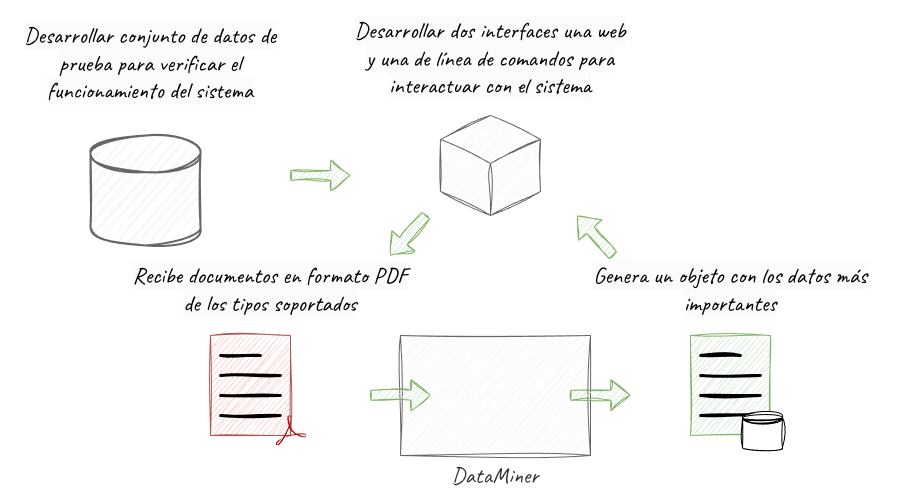
\includegraphics[width=\textwidth]{chapter/1/images/chapter_1.specific}
        \caption{Esquema de los objetivos específicos del sistema}
        \label{fig:chapter_1.specific}
    \end{center}
\end{figure}

Además, el sistema está preparado para introducir nuevas características de una forma sencilla.
Por ejemplo estas son algunas características que pueden ser añadidas fácilmente.

\begin{enumerate}
    \item
    Procesar nuevos formatos de documentos, como pueden ser documentos word, open office, o incluso documentos de video
    o audio
    \item
    Procesar nuevos tipos de documentos, como pueden ser otros tipos de contratos.
\end{enumerate}

    \chapter{Marco teórico}\label{ch:chapter_2}


\section{Código limpio}

\subsection{Introducción histórica}
El concepto de Código Limpio ha sido fundamental en la programación de software desde los primeros días del desarrollo
de software, pero fue articulado y popularizado con gran efecto por Robert C. Martin en su libro~
\cite{book_clean_code_martin_2008}

Este libro se convirtió en una guía esencial para muchos desarrolladores al enfatizar la importancia de escribir código
que no solo funcione, sino que también sea fácil de entender, modificar y mantener.

\subsection{Definición}
El código limpio es aquel que es fácil de entender y fácil de modificar y hace exactamente lo que se espera que haga.
Según Robert C. Martin, el código limpio puede ser leído y mejorado por un desarrollador que no sea su autor original
con un mínimo esfuerzo necesario.

Se caracteriza por su simplicidad, la ausencia de duplicación, la expresión clara de la intención del desarrollador y
la atención a los detalles en el nivel de código.


\section{Arquitectura limpia}

\subsection{Introducción histórica}
En el ámbito del desarrollo de software, la arquitectura de un sistema es crucial para determinar su escalabilidad y
mantenibilidad a largo plazo.

Una de las metodologías que ha cobrado relevancia en este contexto son las ``arquitecturas limpias'', un enfoque para el
diseño de software promovido por Robert C. Martin en su libro Clean Architecture: A Craftsman`s Guide to Software
Structure and Design~\cite{book_clean_code_martin_2017}

\subsection{Definición}
La arquitectura limpia es un estilo de diseño que organiza el sistema de manera que sea independiente de los diferentes
elementos a los que considera detalles de implementación y que son intercambiables unos por otros:

\begin{itemize}
    \item frameworks
    \item interfaces
    \item bases de datos
    \item apis
\end{itemize}

La esencia de esta arquitectura radica en su diagrama de capas, donde cada capa tiene una responsabilidad claramente
definidas y depende solo de las capas más internas.
Esto se logra mediante el principio de inversión de dependencias, lo que significa que los detalles dependen de las
abstracciones y no al contrario.

Existen diferentes implementaciones de ``arquitectura limpia'', cada una con sus características intrínsecas, en este
proyecto hemos decidido implementar una versión de 3 capas.

\begin{figure}[ht]
    \begin{center}
        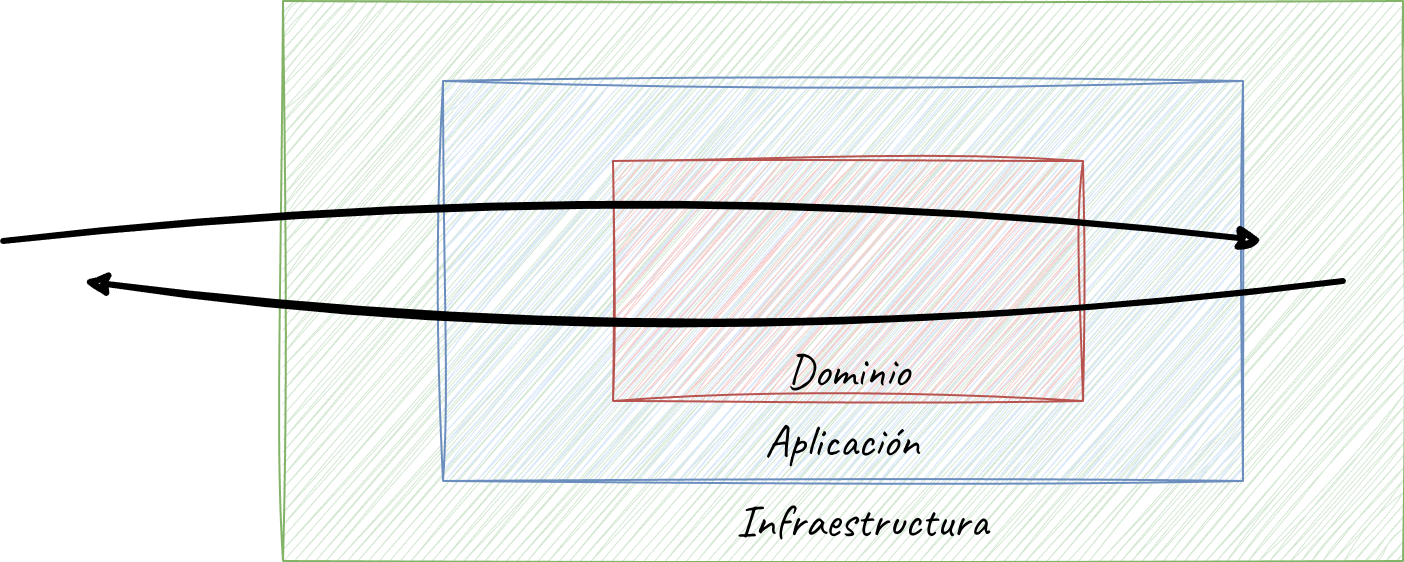
\includegraphics[width=\textwidth]{chapter/2/images/chapter_2.clean_architecture}
        \caption{Esquema de una arquitectura limpia}
        \label{fig:chapter_2.clean_architecture}
    \end{center}
\end{figure}

Representación de las comunicaciones entre capas en una arquitectura limpia.
\colorbox{color_highlight}{@TODO: Insertar figura}

\colorbox{color_highlight}{@TODO: @marlene: mencionales. Aparecen 4 a continuación, por qué?}
\subsubsection*{Dominio}
Es el corazón del modelo de negocio de la aplicación y encapsula la lógica y las reglas del negocio.

Esta capa es fundamentalmente agnóstica respecto a la aplicación de tecnologías externas y se
centra exclusivamente en cómo se comporta el negocio bajo diferentes condiciones y reglas.

Contiene entidades, objetos de valor, y dominios de servicio que representan y operan sobre los
conceptos fundamentales del negocio.

Esta capa debe ser autocontenida y fácilmente testable, aislada de influencias externas como bases de
datos o interfaces de usuario.

\subsubsection*{Aplicación}
La capa de aplicación actúa como un mediador entre la capa de presentación y la capa de dominio, coordinando
las operaciones de alto nivel que involucran múltiples aspectos del dominio.

\subsubsection*{Infraestructura}
La capa de infraestructura proporciona las capacidades tecnológicas necesarias para que las capas de
aplicación y dominio puedan realizar sus funciones sin tener que
preocuparse por los detalles de implementación de la plataforma o los elementos externos.

\subsubsection*{Presentación}
Es responsable de mostrar la información al usuario y de interpretar los
comandos del usuario para que la aplicación pueda entenderlos y actuar en consecuencia.

\colorbox{color_highlight}{@TODO: @marlene: queda mejor si lo redactas como parrafo y no siguiendo ese estilo}


\section{Procesamiento de lenguaje natural}

\subsection{Introducción histórica}
El Procesamiento de Lenguaje Natural o Natural Language Processing (NLP) es un campo que se sitúa en la
intersección de la informática, la inteligencia artificial y la lingüística.

Se dedica al desarrollo de algoritmos y sistemas que permiten a las computadoras entender, interpretar y generar
lenguaje humano de una manera útil y significativa.
La historia del NLP comienza en la década de 1950, marcada por el trabajo pionero de Alan Turing y su famoso
test de Turing, que planteaba la cuestión de si una máquina puede emular el lenguaje humano de manera convincente
(Turing, 1950).

En los años 60 y 70, el enfoque inicial en la traducción automática
, como los esfuerzos del proyecto Georgetown, mostró tanto promesas como limitaciones significativas, lo que llevó a un
reajuste en las expectativas y métodos del campo (Hutchins, 2003).
Con la introducción de la inteligencia artificial (IA) en la década de 1980, surgieron métodos basados primero en reglas
y luego en modelos
estadísticos, culminando con el desarrollo de modelos de aprendizaje automático en la década de 1990 (Manning y Schütze,
1999).

El verdadero cambio paradigmático llegó con el advenimiento de las redes neuronales y el aprendizaje profundo
en la década de 2010.
Este período vio la creación de modelos de lenguaje avanzados, como BERT y GPT, que han revolucionado la capacidad de
las máquinas para procesar el lenguaje con un grado de sutileza y profundidad sin precedentes (Devlin et al., 2019;
Brown et al., 2020).

\subsection{Definición}
El NLP es un campo que combina técnicas de la informática, la inteligencia artificial y la lingüística computacional con
el objetivo de permitir que las máquinas entiendan, interpreten
, manipulen y generen lenguaje humano de manera efectiva y eficiente.

El NLP utiliza algoritmos y modelos matemáticos para abordar diversas tareas relacionadas con el lenguaje, tales como la
traducción automática entre idiomas, la generación de respuestas automáticas
, la extracción de información relevante de textos, el análisis de sentimientos, el reconocimiento de voz, y
la síntesis de habla, entre otros.


\section{Modelos de lenguaje de gran escala (LLMs)}

\subsection{Introducción histórica}
La historia de los LLMs comienza con los primeros modelos estadísticos de lenguaje en
la década de 1980, que utilizaban métodos simples como los modelos de Markov y n-gramas para predecir la probabilidad
de secuencias de palabras (Jelinek, 1997).
Estos métodos, aunque efectivos para algunas tareas básicas, estaban limitados por su incapacidad para capturar
contextos
más largos y por su dependencia de grandes corpus de texto para entrenamiento.

En la década de 2000, con el advenimiento de modelos más sofisticados como los modelos ocultos de Markov
y especialmente las redes neuronales, comenzó a vislumbrarse el
potencial de los modelos de lenguaje más complejos.
Sin embargo, no fue hasta la introducción de las redes neuronales recurrentes (RNN) y, más tarde, las redes neuronales
de memoria a largo plazo (LSTM)
que los investigadores pudieron abordar el problema del ''desvanecimiento del gradiente''
y mejorar significativamente la capacidad de los
modelos para aprender dependencias a largo plazo en el texto (Hochreiter Schmidhuber, 1997).

\subsubsection*{La revolución de los transformers}
El verdadero cambio paradigmático llegó en 2017 con el desarrollo de la arquitectura
Transformer por Vaswani et al.
Esta arquitectura introdujo el mecanismo de atención, que permite a los modelos ponderar diferentes partes de la entrada
de texto de manera dinámica, mejorando la capacidad de los modelos para manejar secuencias de texto largas y complejas (
Vaswani et al., 2017).

\colorbox{color_highlight}{@TODO: @marlene Transformers términos en inglés van en itálicas}

BERT, desarrollado por Google en 2018, y GPT, desarrollado por OpenAI, son ejemplos de
cómo los Transformers han sido adaptados para crear modelos que
no solo entienden el contexto de una palabra en función de su posición en una frase, sino en todo
el texto, permitiendo un entendimiento contextual mucho más rico (Devlin et al., 2019; Radford et al., 2018).

\subsection{Definición}
Los Modelos de Lenguaje de Gran Escala (LLMs) son sistemas
avanzados de inteligencia artificial diseñados para entender, generar y
manipular el lenguaje humano de manera coherente y contextualizada. Estos
modelos son entrenados en vastos conjuntos de datos textuales que abarcan una amplia variedad de temas, lo que les
permite desarrollar un conocimiento extenso sobre el lenguaje y sus usos prácticos.

Funcionan principalmente a través de técnicas de aprendizaje
profundo, especialmente usando arquitecturas como las de Transformers,
que permiten a los modelos captar relaciones complejas y contextos a largo plazo dentro de los textos. Este enfoque les
otorga la capacidad de generar respuestas, completar textos,
traducir entre idiomas, resumir información y responder preguntas con un alto grado de precisión y relevancia.

\subsection{Principales modelos}

\colorbox{color_highlight}
{@TODO: @marlene: puedes hacer un resumen de estos modelos. Creo que no hace falta que coloques los código de ejemplos.
Quizás
para un anexo}
\subsubsection*{OpenAI GPT}
ChatGPT es un avanzado modelo de lenguaje desarrollado por OpenAI,
basado en la arquitectura GPT (Generative Pre-trained Transformer).

Es uno de los modelos más reconocidos en la actualidad.
Aunque es un modelo privado, OpenAI ofrece acceso a través de una API de pago que incluye una capa gratuita limitada.

ChatGPT ofrece varios modelos, cada uno con un esquema de precios que varía según
su complejidad.
Una de las principales ventajas de este servicio es que proporciona una solución integral "plug-and-play", es decir, no
requiere instalación ni configuración adicional por parte del usuario.

A continuación un ejemplo de una llamada a esta API.


\subsubsection*{Hugging Face's Transformers}
Hugging Face's Transformers
es una biblioteca de procesamiento de lenguaje natural (NLP) que simplifica el uso de modelos de aprendizaje profundo
basados en la arquitectura Transformer.

Esta biblioteca ofrece una amplia variedad de modelos pre entrenados desarrollados por la comunidad
para fines específicos, además de la posibilidad de entrenar modelos personalizados.


Sin embargo, los modelos disponibles en Hugging Face suelen ser menos potentes que los modelos más
avanzados disponibles a través de plataformas como ChatGPT. ChatGPT ofrece
modelos con capacidades superiores, lo que puede ser una
consideración importante dependiendo de los requisitos específicos del proyecto.

\subsubsection*{Otros}
Además de OpenAI y Hugging Face, existen varias otras plataformas que ofrecen modelos de lenguaje
grande (LLM) para desarrolladores interesados en incorporar capacidades
avanzadas de procesamiento de lenguaje natural en sus aplicaciones. Entre
estas plataformas destacan Google AI, Facebook AI, NVIDIA NeMo y Microsoft AI, entre otras cada una con sus propios
enfoques y modelos distintivos.

    \chapter{Metodología}\label{ch:chapter_3}


\section{Programación extrema}

La Programación Extrema o \textit{extreme programming} (XP) es una metodología ágil de desarrollo de software que se
enfoca en mejorar la calidad del software y la capacidad de respuesta a las necesidades cambiantes del cliente.
Introducida por Kent Beck en el libro \textit{Extreme Programming Explained: Embrace Change}~\cite{book_beck_1999},
XP promueve la colaboración intensa entre los desarrolladores y los clientes, ciclos de
desarrollo cortos y frecuentes, y la entrega continua de pequeñas mejoras.

Una de las principales ventajas de XP es su capacidad para adaptarse rápidamente a los cambios en los requisitos del
cliente, lo que facilita que el producto final satisfaga las necesidades del negocio.


\section{Desarrollo dirigido por pruebas}

El desarrollo dirigido por pruebas o \textit{test driven development} (TDD) es una práctica de desarrollo de software.
Este enfoque fue popularizado por Kent Beck, uno de los pioneros de las metodologías ágiles, en su libro
\textit{Test Driven Development: By Example}~\cite{book_beck_2003}.
TDD se basa en ciclos cortos de desarrollo donde se escribe una prueba, se implementa el código necesario para pasar la
prueba y luego se refactoriza el código para mejorar su estructura sin cambiar su comportamiento.


\section{Kanban}
Es un método de gestión de proyectos y flujo de trabajo que se originó en la industria manufacturera japonesa,
específicamente en Toyota, como una forma de mejorar la eficiencia de la producción~\cite{book_anderson_2010}.
El término significa ``tarjeta visual` en japonés, y el método se basa en el uso de tarjetas visuales para
representar tareas en un tablero, permitiendo a los equipos ver el estado del trabajo en progreso de un
vistazo.

Kanban promueve la mejora continua, la flexibilidad y la eficiencia, ayudando a los equipos a gestionar el flujo de
trabajo y a identificar cuellos de botella rápidamente.

En la figura~\ref{fig:chapter_3.kanban} aparece el tablero kanban utilizado en el desarrollo de este proyecto.

\begin{figure}
    \begin{center}
        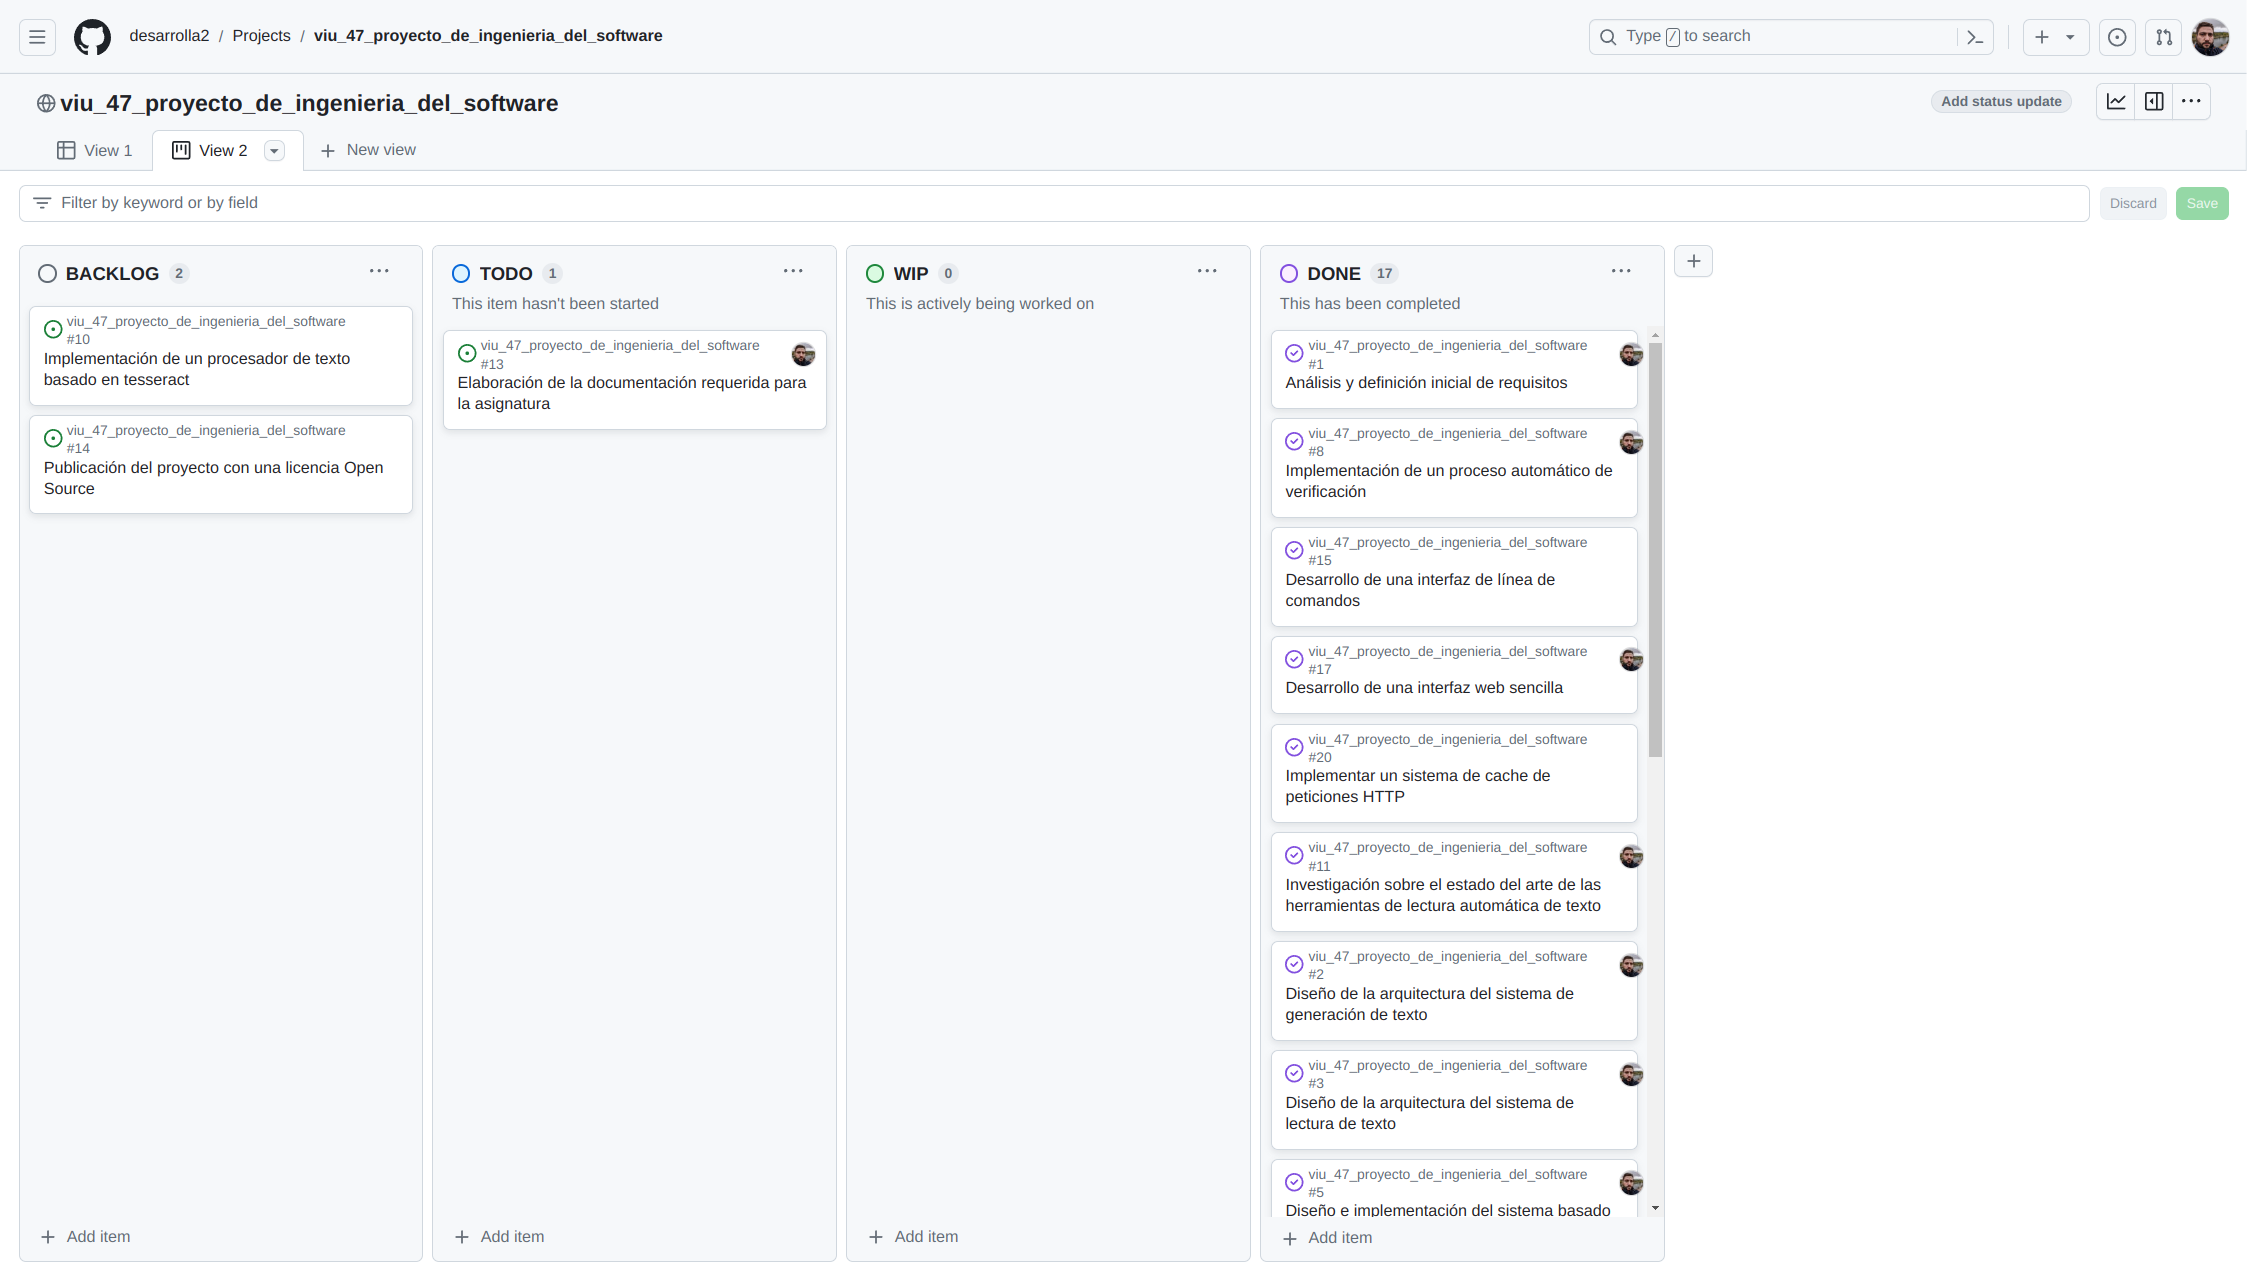
\includegraphics[width=\textwidth]{./chapter/3/images/chapter_3.kanban}
        \caption{Captura de pantalla del tablero kanban del proyecto}
        \label{fig:chapter_3.kanban}
    \end{center}
\end{figure}
    \chapter{Desarrollo}\label{ch:chapter_4}

\begin{comment}
    En este apartado se describe detalladamente el proceso de implementación y desarrollo de tu proyecto. En esta
    sección, se proporciona información sobre cómo se han llevado a cabo las etapas de diseño, programación, pruebas y
    evaluación de tu solución. A continuación, se presentan algunos elementos típicos que se incluyen en el apartado de
    desarrollo:

    Diseño del sistema: Describe el diseño de tu sistema o solución informática. Explica la arquitectura general, los
    componentes principales y las interacciones entre ellos. Puedes utilizar diagramas, esquemas o modelos para ilustrar
    visualmente el diseño del sistema.

    Tecnologías utilizadas: Indica las tecnologías específicas que has utilizado en tu desarrollo, como lenguajes de
    programación, frameworks, librerías, sistemas operativos, bases de datos, herramientas de desarrollo, entre otros.
    Describe cómo se han aplicado estas tecnologías en tu proyecto.

    Desarrollo de software: Explica el proceso de desarrollo de software que has seguido. Puedes mencionar cómo se ha
    realizado la planificación, el seguimiento y la gestión del proyecto. Detalla las etapas de análisis, diseño,
    implementación y pruebas del software.

    Implementación y programación: Describe cómo has implementado tu solución informática.. Proporciona ejemplos de
    código relevante para ilustrar las características principales de tu implementación.

    Pruebas y evaluación: Detalla las pruebas realizadas para verificar el correcto funcionamiento de tu solución.
    Explica los casos de prueba utilizados, los resultados obtenidos y cómo se han abordado los problemas o errores
    identificados. Si has realizado pruebas de rendimiento, seguridad u otros aspectos, también inclúyelos en esta
    sección.

    Iteraciones y mejoras: Si has realizado iteraciones o mejoras en el proceso de desarrollo, menciona los cambios
    realizados y las razones detrás de ellos.

    Consideraciones técnicas: Si hay consideraciones técnicas importantes relacionadas con tu desarrollo, como
    requisitos de hardware o restricciones de recursos, menciónalas en esta sección. Explica cómo has abordado estos
    desafíos técnicos y cómo han influido en el desarrollo de tu proyecto.

\end{comment}


\section{Descripción del proyecto}

Hemos creado una solución tecnológica con dos interfaces: una web y una de línea de comandos, que recibe documentos
en formato PDF y extrae de ellos la información que contienen.


\section{Alcance}

El software que hemos desarrollado hasta ahora sirve como una base conceptual y prototipo inicial.
Se ha desarrollado una herramienta que es capaz de procesar datos de contratos de los siguientes tipos:

\begin{enumerate}
    \item Contrato de arrendamiento de vivienda entre particulares
    \item Contrato de compraventa de vehículo entre particulares
\end{enumerate}


\section{Tecnologías utilizadas}
El proyecto hace uso de una variedad de tecnologías modernas para asegurar un desarrollo eficiente,
una implementación robusta y una experiencia de usuario óptima.
\colorbox{color_highlight}{@TODO: @marlene:} cómo lo evaluaste?

A continuación, se describen las principales tecnologías utilizadas en
el proyecto, categorizadas en distintas áreas según su propósito y aplicación.

\colorbox{color_highlight}{@TODO: @marlene:} colocar referencias

\subsection*{Backend}

*PHP

Es un lenguaje de scripting de propósito general que está especialmente diseñado para el desarrollo web.
PHP permite crear aplicaciones web dinámicas y está ampliamente soportado en servidores web.

Symfony

Symfony es un framework PHP ampliamente utilizado para desarrollar aplicaciones web.
Ofrece una arquitectura robusta y flexible, que facilita el desarrollo de aplicaciones mantenibles y escalables.

Twig

Twig es un motor de plantillas para PHP, utilizado principalmente en proyectos basados en
Symfony.
Facilita la creación de vistas dinámicas y mantenibles, separando la lógica de presentación del código de negocio.

\subsection*{Frontend}

HTML5

Es el estándar de marcado para crear páginas web.
HTML5 introduce nuevas funcionalidades como elementos semánticos y multimedia, mejorando la accesibilidad y la
interoperabilidad de las páginas web.

CSS3

Es la tecnología de estilos para el diseño visual.
CSS3 permite aplicar estilos complejos y responsivos a los elementos HTML, mejorando la presentación y la experiencia
del usuario.

JavaScript

Es el lenguaje de programación para la interactividad del lado del cliente.
JavaScript permite crear experiencias de usuario dinámicas y responsivas, manejando eventos y actualizando el contenido
de la página sin recargar.

Bootstrap

Es un framework de front-end que facilita el diseño de sitios y aplicaciones web
responsivas y móviles.
Bootstrap proporciona una colección de componentes CSS
y JavaScript predefinidos que aceleran el desarrollo de interfaces de usuario atractivas.

Font Awesome

Es una biblioteca de iconos vectoriales y herramientas que proporciona una amplia gama de
iconos escalables y personalizables para su uso en proyectos web.
Facilita la inclusión de iconos de alta calidad sin depender de imágenes.

\subsection*{Gestión de dependencias}

Composer

Es una herramienta de gestión de dependencias para PHP, que
permite declarar las bibliotecas de las que depende tu proyecto
y las gestiona.
Composer asegura que las versiones correctas de las bibliotecas se instalen y mantengan actualizadas.

\subsection*{Control de versiones}

Git

Es un sistema de control de versiones distribuido, diseñado para manejar todo, desde proyectos
pequeños hasta muy grandes con rapidez y eficiencia.
Git permite a los desarrolladores colaborar de manera efectiva, rastreando cambios y gestionando ramas y fusiones.


GitHub

GitHub es una plataforma de hospedaje de repositorios Git.
Proporciona herramientas para la colaboración, la revisión de código y la gestión de proyectos, facilitando el trabajo
en equipo y la integración continua.

\subsection*{Automatización}

Make

Make es una herramienta de automatización de tareas que utiliza archivos Makefile para definir y ejecutar tareas de
construcción y gestión de proyectos.
Facilita la automatización de tareas repetitivas y la configuración del entorno de desarrollo.

\subsection*{Pruebas}

PHPUnit

PHPUnit es un marco de pruebas unitarias para PHP. Permite a los desarrolladores escribir y ejecutar pruebas
automatizadas
para asegurar que el código se comporta como se espera, facilitando el desarrollo de software de alta calidad.

GitHub Actions

Es una plataforma de integración continua que permite automatizar flujos de trabajo directamente desde GitHub.
GitHub Actions facilita la configuración de pipelines de CI/CD, ejecutando pruebas y despliegues automáticamente con
cada cambio en el repositorio.

\subsection*{Contenerización}

Docker

Docker es una plataforma que permite desarrollar, enviar y ejecutar aplicaciones dentro de
contenedores.
Proporciona un entorno consistente para el desarrollo, pruebas y despliegue, asegurando que las aplicaciones funcionen
de manera idéntica en diferentes entornos.

Docker Compose

Docker Compose es una herramienta para definir y ejecutar aplicaciones Docker multi-contenedor.
Permite orquestar varios servicios que componen una aplicación, facilitando
la configuración y gestión de entornos de desarrollo complejos.

\subsection*{Logs}

Monolog

Monolog es una biblioteca de logging para PHP. Permite enviar registros a varios destinos, como archivos, bases de datos
y servicios de terceros, facilitando la monitorización y depuración de aplicaciones.

Elastic Search

Elasticsearch es un motor de búsqueda y análisis de texto completo basado en Lucene.
Permite almacenar, buscar y analizar grandes volúmenes de datos en tiempo real.

Logstash

Logstash es una herramienta de procesamiento de datos que ingesta, transforma y envía datos a varios
destinos.
Es parte del paquete Elasticsearch, Logstash, Kibana (ELK) y facilita la recolección y procesamiento de logs.

Kibana

Kibana es una herramienta de visualización de datos que trabaja en conjunto con Elasticsearch.
Permite a los usuarios crear gráficos y dashboards interactivos para visualizar y analizar los datos de logs almacenados
en Elasticsearch.

\subsection*{Componente Generator}

Pdf to text

Pdf to Text es una herramienta que convierte documentos PDF en texto plano.
Permite extraer el contenido textual de archivos PDF, lo cual es útil para la posterior manipulación y análisis de
datos.

\subsection*{Componente Reader}

Symfony HttpClient

Symfony HttpClient es un cliente HTTP flexible y eficiente para PHP. Permite realizar solicitudes HTTP a servicios
externos, manejar respuestas y gestionar errores de manera sencilla y eficaz.

Symfony Cache

Symfony Cache es un componente de Symfony que proporciona una implementación robusta y flexible para el almacenamiento
en caché.
Permite mejorar el rendimiento de la aplicación mediante el almacenamiento temporal de datos, reduciendo la carga en los
recursos externos.

API Open AI

La API de OpenAI proporciona acceso a modelos avanzados de procesamiento de lenguaje natural.
Permite integrar capacidades de IA en la aplicación, como la generación de texto y el análisis de datos, mejorando las
funcionalidades y experiencias del usuario.


\colorbox{color_highlight}{@TODO: @marlene:}
En cuanto a los datos, los generaste manual. No hay forma de generar datos sintéticos? Se podrían generar 100 o 1000
documentos? Sino, hay que justificarlo bien.

\colorbox{color_highlight}{@TODO: @marlene:}
Vale, veo que si usas el LLM de chatgpt. Eso es algo que no me había quedado claro de la memoria. Sin embargo, aún no
tengo del todo claro qué generas a partir del PDF que recibes. Puedes ejecutar tu herramienta con un contrato? Estás
usando el LLM para extraer los datos del contenido del PDF? Otra pregunta, qué modelo de chatgpt estás usando? Y puedes
mandar el prompt que usaste?


\section{Arquitectura del sistema}
Se pretende diseñar un sistema basado en dos componentes cada uno de los cuales es fácilmente extensible, permitiéndole
añadir funcionalidades específicas para cada caso de uso.

Hemos diseñado el sistema con dos componentes principales, el Generator y el Reader.

\colorbox{color_highlight}{@TODO: @marlene:} recuerda referenciar y explicar las figuras

\begin{figure}
    \centering
    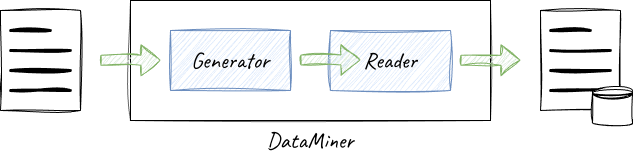
\includegraphics
    {./chapter/4/images/ad_4nxfvsrqaa0z4oog6ioupbhm9di1ks0uugteour8yll1z9polcxzput4la1osaqqlp61xyowlcejwkesovongxvd1rop2gxft}
    \caption{}
    \label{fig:ad_4nxfvsrqaa0z4oog6ioupbhm9di1ks0uugteour8yll1z9polcxzput4la1osaqqlp61xyowlcejwkesovongxvd1rop2gxft}
\end{figure}

Esquema de la arquitectura del sistema con sus principales componentes.

Esta estructura no solo promueve la eficiencia y adaptabilidad, sino que también asegura la calidad y mantenibilidad del
código, permitiendo que el sistema se ajuste y evolucione según las necesidades futuras.

\subsection*{Generator}
Este componente sirve como el motor inicial en el proceso, encargado de convertir documentos de cualquier formato a
texto plano. Se compone de tres elementos específicos y un orquestador que coordina la secuencia de operaciones.

\begin{figure}
    \centering
    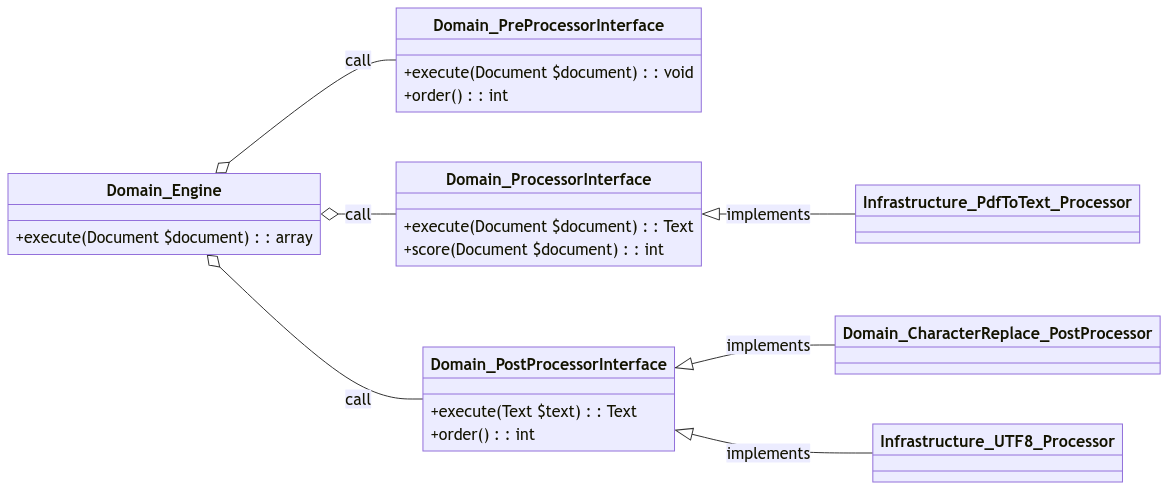
\includegraphics
    {./chapter/4/images/ad_4nxcpbcugaqoykyq7hbpnr9p7_uswyuzipkcqvfkgc1fhoclp9cwrzu6zkoszpxi3zqsthvvftxotwhksqawgubuwqffg5gxn}
    \caption{}
    \label{fig:ad_4nxcpbcugaqoykyq7hbpnr9p7_uswyuzipkcqvfkgc1fhoclp9cwrzu6zkoszpxi3zqsthvvftxotwhksqawgubuwqffg5gxn}
\end{figure}

Diagrama UML del componente generator.

\subsubsection*{Preprocesadores}
Estos componentes ajustan el documento original para facilitar su análisis. Realizan modificaciones como el ajuste de
contraste para optimizar la efectividad del reconocimiento óptico de caracteres (OCR), mejorando la legibilidad del
texto.

\begin{figure}
    \centering
    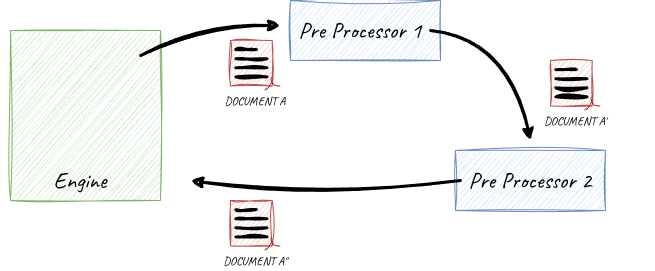
\includegraphics
    {./chapter/4/images/ad_4nxccemzz1bxsroksvslihdkre9_b2-yqr2hu4hmvwfblvicw_lzbshudm5upl70uk6mxjhlpzvaa8b79oba_npzrpimoggwd}
    \caption{}
    \label{fig:ad_4nxccemzz1bxsroksvslihdkre9_b2-yqr2hu4hmvwfblvicw_lzbshudm5upl70uk6mxjhlpzvaa8b79oba_npzrpimoggwd}
\end{figure}

Comunicación del Engine con los pre procesadores definidos.

En esta implementación no se ha desarrollado ningún Pre-procesador.

\subsubsection*{Procesadores}
Actúan como el núcleo del Generator, donde se realiza la conversión efectiva del documento a texto. Funcionan mediante
un sistema competitivo donde varios procesadores evalúan su propia aptitud para manejar el documento en cuestión,
seleccionando el más adecuado para llevar a cabo la tarea.

Este enfoque modular y competitivo asegura que el procesamiento del texto sea no solo eficiente, sino también
extremadamente flexible, adaptándose a las variaciones en la naturaleza de los documentos procesados.

\begin{figure}
    \centering
    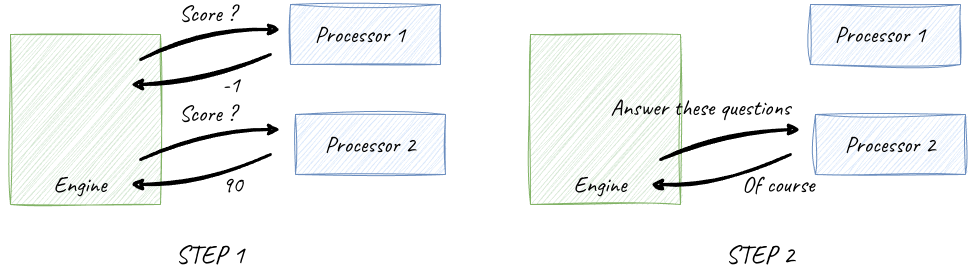
\includegraphics
    {./chapter/4/images/ad_4nxflatsoejeb4h5hddo8a4otwjmcaznrikw1gvyzmtafloyas7kuglrhwlolub-qvwzl1ckw6ugltisracet07luw4uskwmx}
    \caption{}
    \label{fig:ad_4nxflatsoejeb4h5hddo8a4otwjmcaznrikw1gvyzmtafloyas7kuglrhwlolub-qvwzl1ckw6ugltisracet07luw4uskwmx}
\end{figure}

Comunicación del Engine con los procesadores definidos.

En la actual implementación, hemos desarrollado un único procesador especializado en transformar documentos PDF a
texto. Este procesador utiliza la utilidad de línea de comandos `pdftotext` para llevar a cabo la conversión (Glyph \&
Cog, 2023).

\subsubsection*{Postprocesadores}
Estos componentes perfeccionan el texto generado, eliminando errores como caracteres no UTF-8 y espacios en blanco
innecesarios, lo que mejora significativamente la calidad del texto resultante. En esta implementación, se han
desarrollado varios post-procesadores:

\begin{itemize}
    \item
    Word Limit PostProcessor: Se detectó que los elementos de interés, como nombres, documentos de identidad y fechas de
    contratos, típicamente aparecen en las primeras páginas. Este procesador limita el análisis a las primeras N
    palabras del documento.
    \item UTF8 PostProcessor: Implementado tras detectar caracteres no UTF-8 en algunos documentos, este post-procesador
    elimina dichos caracteres.
    \item Character Replace PostProcessor: Desarrollado para eliminar caracteres específicos que complicaba las pruebas.
\end{itemize}

\subsubsection*{Engine}
Este es el orquestador del componente, encargado de hacer las llamadas a los demás elementos registrados en la
aplicación. Coordina el flujo entre los pre-procesadores, procesadores y post-procesadores para asegurar que el
documento sea procesado de manera correcta.

\subsection*{Reader}
El componente Reader juega un papel crucial en el proceso de interpretación y procesamiento del texto plano obtenido a
partir de la salida del componente Generator anterior..

Funciona mediante un sistema de procesadores organizados en una única capa, que opera bajo un mecanismo competitivo
similar al del componente Generator. En este sistema, los procesadores compiten entre sí para determinar cuál es el más
adecuado para analizar y extraer la información estructurada necesaria del texto.

\begin{figure}
    \centering
    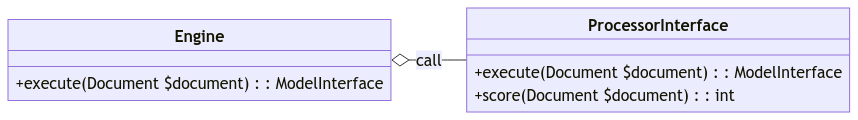
\includegraphics
    {./chapter/4/images/ad_4nxcg3r2qv9xc3mw0lynfkpfwfmxpbrpvfhfpr7-3idtd0eopjq9nsbhnvqcgq5hz9hwcy4jam9vqvffwys6jvo_a20paqxml}
    \caption{}
    \label{fig:ad_4nxcg3r2qv9xc3mw0lynfkpfwfmxpbrpvfhfpr7-3idtd0eopjq9nsbhnvqcgq5hz9hwcy4jam9vqvffwys6jvo_a20paqxml}
\end{figure}

Diagrama UML del componente Reader.

\subsubsection*{Procesadores}
Cada uno de estos procesadores es invocado secuencialmente para evaluar su idoneidad en el manejo del documento
específico..

Una vez seleccionado, el procesador elegido procede a ejecutar una serie de tareas que incluyen la identificación y
extracción de entidades clave. En esta implementación, se han desarrollado los siguientes procesadores:

\begin{itemize}
    \item Residential Lease Processor: Evalúa si el documento se trata de un contrato de alquiler de vivienda entre
    particulares. En caso afirmativo, extrae la información más relevante del mismo, como los nombres de los
    arrendadores, los arrendatarios y la fecha del contrato.
    \item Vehicle Sale And Purchase Processor: Evalúa si el documento se trata de un contrato de compraventa de
    vehículos
    entre particulares. En caso afirmativo, extrae la información más relevante del mismo, como los nombres de los
    compradores y vendedores y la fecha de la transacción.
\end{itemize}

\subsubsection*{Engine}
Este es el orquestador del componente, encargado de hacer las llamadas a los demás elementos registrados en la
aplicación, en este caso únicamente los procesadores.

\section*{Pruebas}
Las pruebas en este proyecto son fundamentales para asegurar que la tecnología funciona conforme a las expectativas y
requisitos establecidos. Para garantizar una validación exhaustiva y precisa, se ha diseñado cuidadosamente un sistema
de pruebas descrito a continuación.

\subsection*{Construcción del conjunto de datos de prueba}

\colorbox{color_highlight}{@TODO: @marlene:} menciona el tamaño del dataset
El proceso para encontrar un conjunto de datos de prueba fue complejo, ya que no se encontraron conjuntos de datos de
fuentes abiertas que cumplieran con los requisitos necesarios..

La mayoría de estos conjuntos se distribuyen anonimizados, y nuestra tecnología necesita identificar y extraer
principalmente datos de carácter personal, como nombres, documentos de identidad, direcciones, fechas, importes, números
de cuentas bancarias, entre otros.

Finalmente, se construyó manualmente un conjunto de datos de prueba utilizando modelos de documentos encontrados en
internet, así como contratos reales a los que tuvimos acceso..

Este conjunto de datos se compone de tres subconjuntos:


INSERTAR TABLA

El siguiente paso fue modificar todos los documentos para que todos los datos de carácter personal fueran aleatorios y
no correspondiera a personas reales. Este proceso aseguró la privacidad y cumplió con las normativa de protección de
datos.

Para facilitar la modificación y manejo de estos documentos, se guardaron en formato Markdown, lo que permitió una
edición más rápida en el propio editor de código.

Dado que la entrada del sistema acepta documentos en formato PDF, se desarrolló un pequeño script para convertir cada
documento Markdown en PDF. Este script utiliza plantillas LaTeX para introducir variabilidad en el formato de los
documentos, asegurando una mayor robustez en las pruebas del sistema.

\begin{figure}
    \centering
    
\includegraphics
    {./chapter/4/images/ad_4nxecxswzqiymihljxkmhkqchczjiqhus6eig0e_yq0a6yb2hktidggwooz_rykz6geygyfckw5z2v-cib6abuod5vrhxfggw}
    \caption{}
    \label{fig:ad_4nxecxswzqiymihljxkmhkqchczjiqhus6eig0e_yq0a6yb2hktidggwooz_rykz6geygyfckw5z2v-cib6abuod5vrhxfggw}
\end{figure}

Este enfoque en la creación del conjunto de datos de prueba garantiza que el sistema pueda ser evaluado de manera
exhaustiva y precisa, cubriendo diversos escenarios y tipos de documentos relevantes para la tecnología desarrollada.

\subsection*{Pruebas automáticas}
Las pruebas automáticas son esenciales para garantizar la calidad y la robustez del software. Permiten verificar que el
código se comporta como se espera, identificar errores de manera temprana y asegurar que las nuevas funcionalidades no
introduzcan fallos en el sistema existente..

En este proyecto, se han implementado varios tipos de pruebas automáticas, cada una con un enfoque diferente para cubrir
todas las facetas del desarrollo y la implementación del software.

\subsubsection*{Pruebas unitarias}
Las pruebas unitarias se centran en verificar la funcionalidad de componentes individuales del sistema, como funciones o
métodos. Estas pruebas son cruciales para asegurar que cada parte del código funciona correctamente en aislamiento.

Se utilizan frameworks de pruebas, como PHPUnit, para automatizar estas pruebas y hacerlas repetibles y confiables.

\begin{figure}
    \centering
    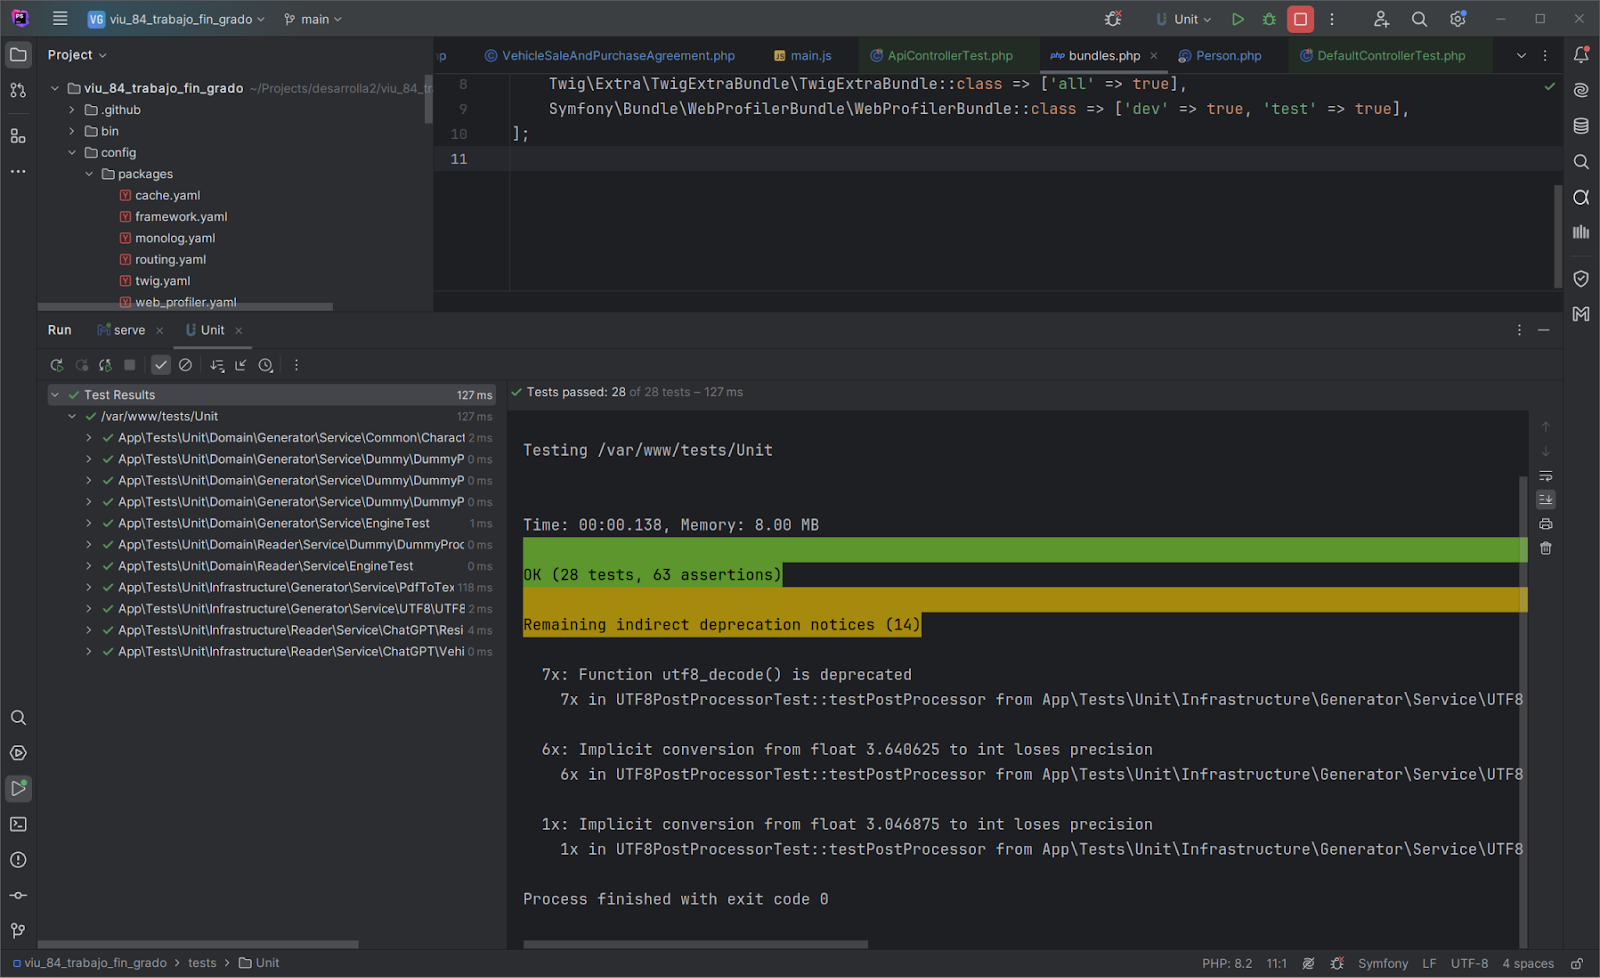
\includegraphics
    {./chapter/4/images/ad_4nxf9wl5tpdrrtr3bqpnmamma-tjdxo4hakx3gbtkr7xbxwuphltuchx5wkg5qz1sviw7hdopfifg-etui-spj9crpegapnd0}
    \caption{}
    \label{fig:ad_4nxf9wl5tpdrrtr3bqpnmamma-tjdxo4hakx3gbtkr7xbxwuphltuchx5wkg5qz1sviw7hdopfifg-etui-spj9crpegapnd0}
\end{figure}

Pruebas unitarias ejecutadas desde un entorno de desarrollo integrado

\subsubsection*{Pruebas funcionales}
Las pruebas funcionales evalúan el sistema desde el punto de vista del usuario final, verificando que las
funcionalidades del software se comportan como se espera cuando se integran varios componentes.

\begin{figure}
    \centering
    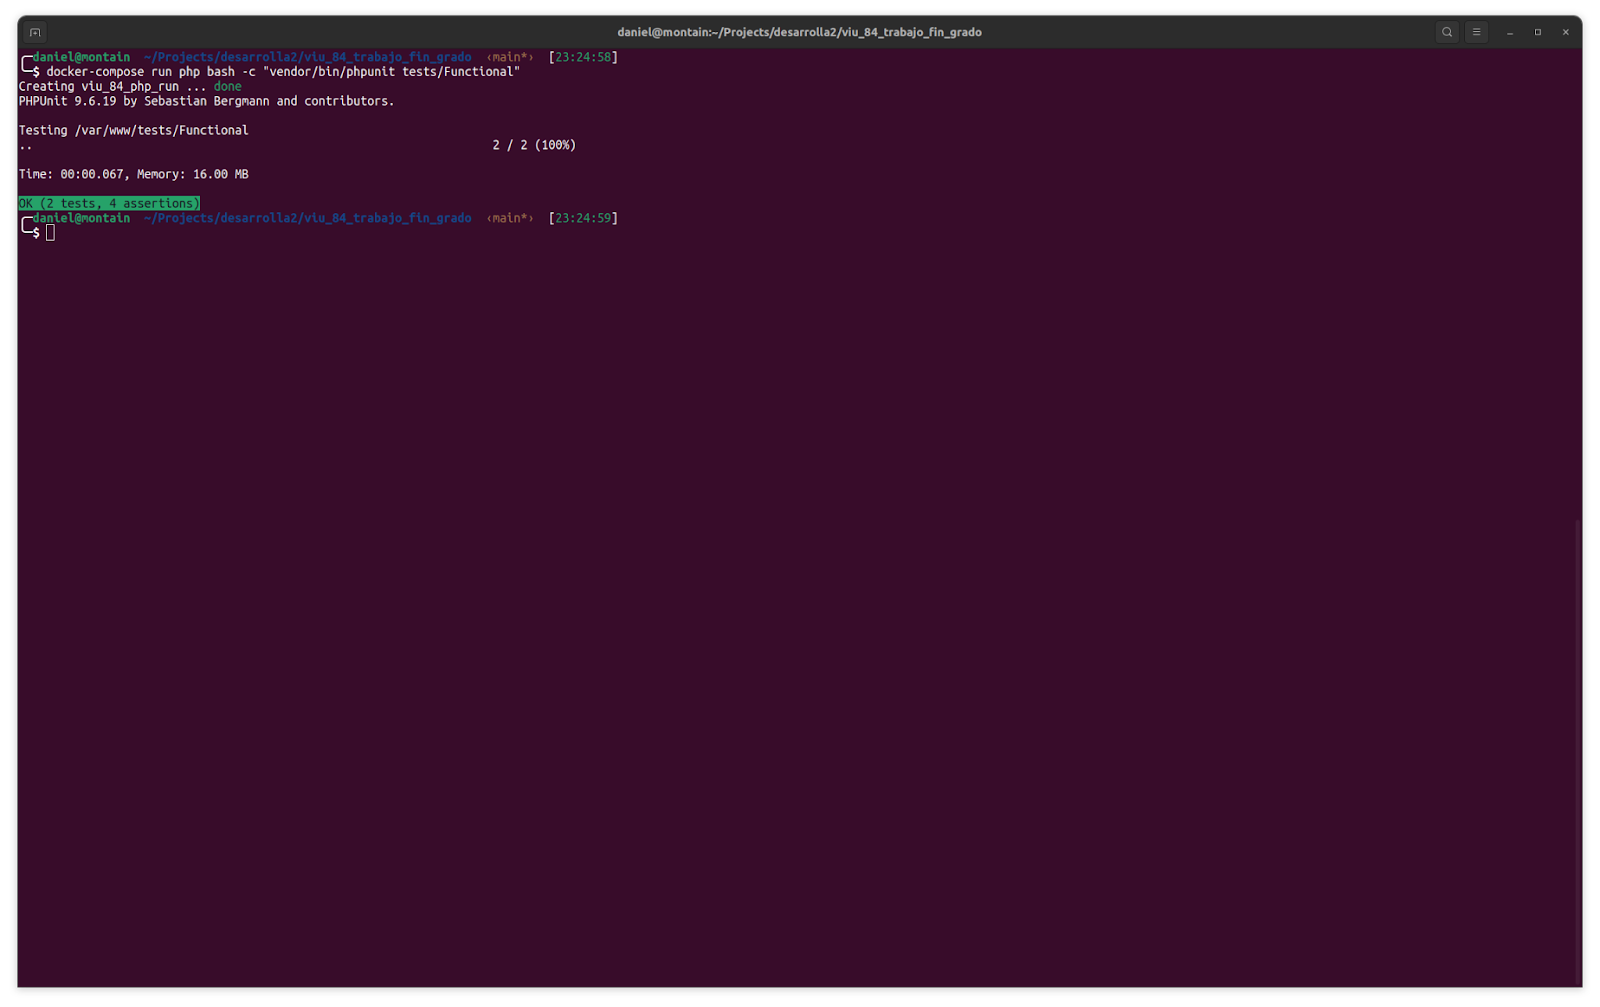
\includegraphics
    {./chapter/4/images/ad_4nxdjm3roncapqpcqzlpzzayuchtishsa3qakfjkye76hnjfezwpd02lbc5ipmjkrhfaqwtwmte-fc_rb67mnqawk_ylrrbdp}
    \caption{}
    \label{fig:ad_4nxdjm3roncapqpcqzlpzzayuchtishsa3qakfjkye76hnjfezwpd02lbc5ipmjkrhfaqwtwmte-fc_rb67mnqawk_ylrrbdp}
\end{figure}

Pruebas funcionales ejecutadas desde la línea de comandos

\subsection*{Integración continua}
La integración continua es una práctica esencial en el desarrollo de software moderno, que implica la integración
frecuente del trabajo de los desarrolladores en un repositorio compartido, normalmente programando la ejecución
automática de los test en un servidor de integración continua, cada vez que se añade un commit al repositorio.

En este proyecto, hemos implementado la integración continua utilizando GitHub Actions, un servicio de automatización
que permite crear flujos de trabajo personalizados para compilar, probar y desplegar código directamente desde GitHub.

\begin{figure}
    \centering
    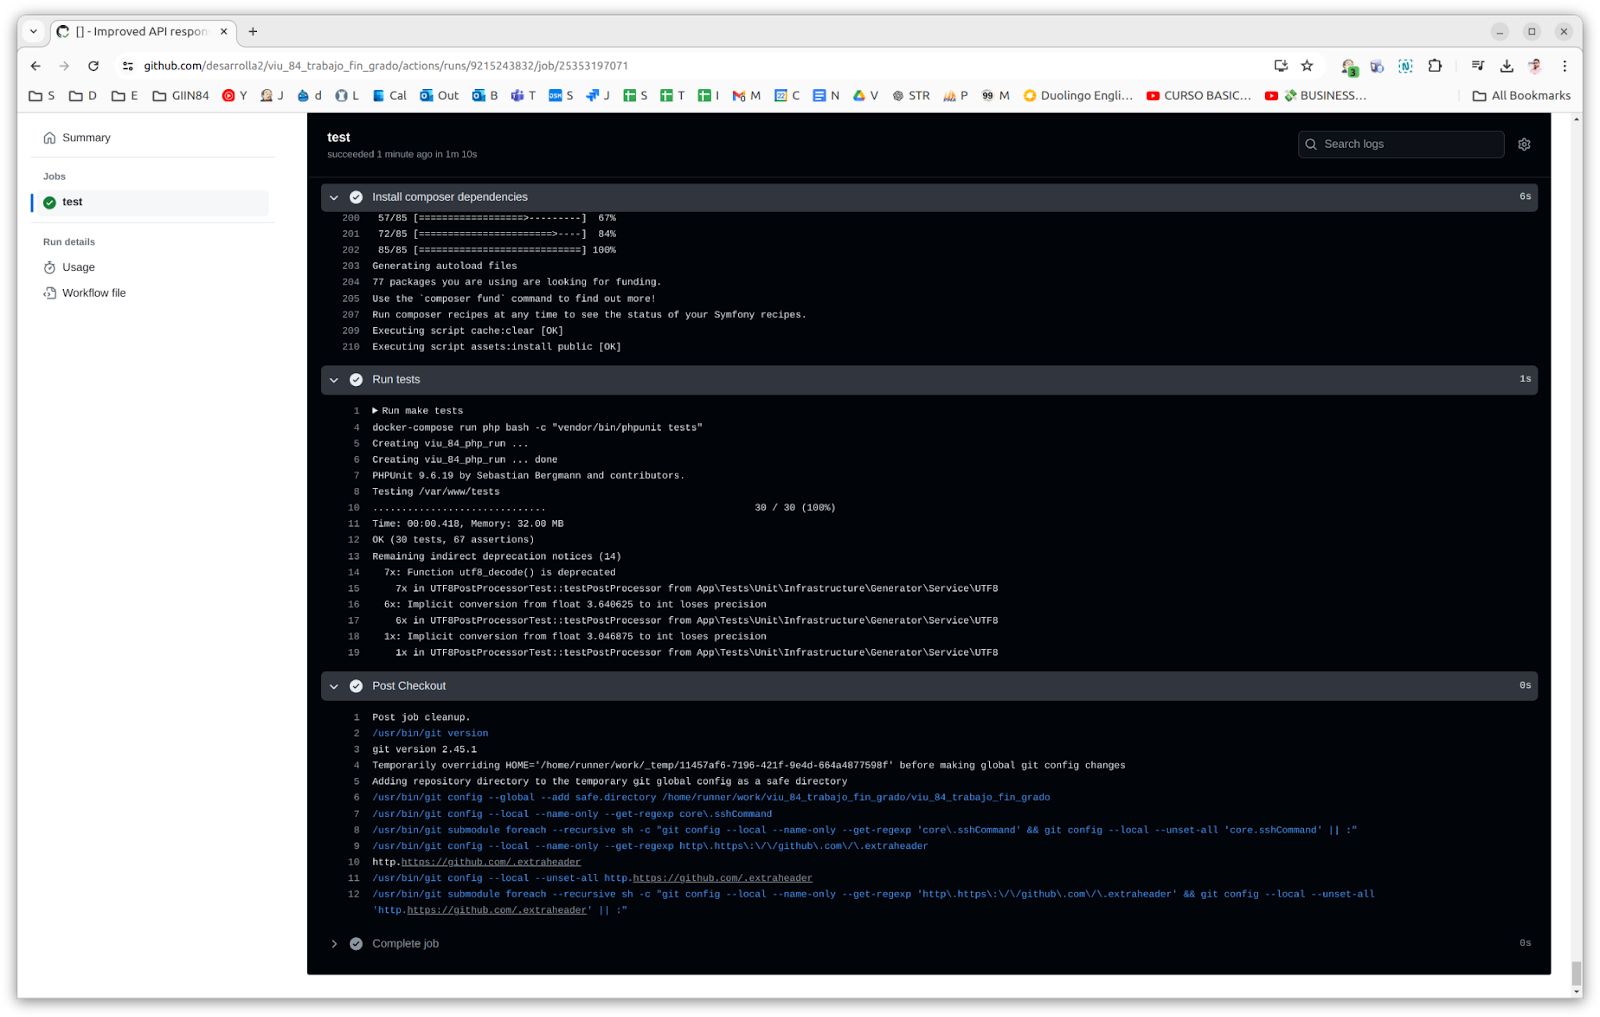
\includegraphics
    {./chapter/4/images/ad_4nxdvwcz-hxwpamvogmkpwsiwmslmhgbyffk5opiurddtpas2hrsdbgqev6iyg4zlpo67ljzpo0_bovbcxojsomq7dt3vxdvv}
    \caption{}
    \label{fig:ad_4nxdvwcz-hxwpamvogmkpwsiwmslmhgbyffk5opiurddtpas2hrsdbgqev6iyg4zlpo67ljzpo0_bovbcxojsomq7dt3vxdvv}
\end{figure}

Pruebas de Integración continua realizada en GitHub actions.

\section*{Interfaces de usuario}
Aunque el objetivo principal de este trabajo es desarrollar una tecnología, flexible, extensible y que pueda ser
fácilmente integrada en otros sistemas, se han implementado dos tipos de interfaces sencillas, que permiten demostrar el
correcto funcionamiento de la tecnología.

\subsection*{Interfaz de línea de comandos}
La interfaz de línea de comandos es una herramienta para desarrolladores y administradores del sistema. Permite ejecutar
comandos y scripts de manera directa, facilitando la automatización de tareas y la integración con otros sistemas.

\begin{figure}
    \centering
    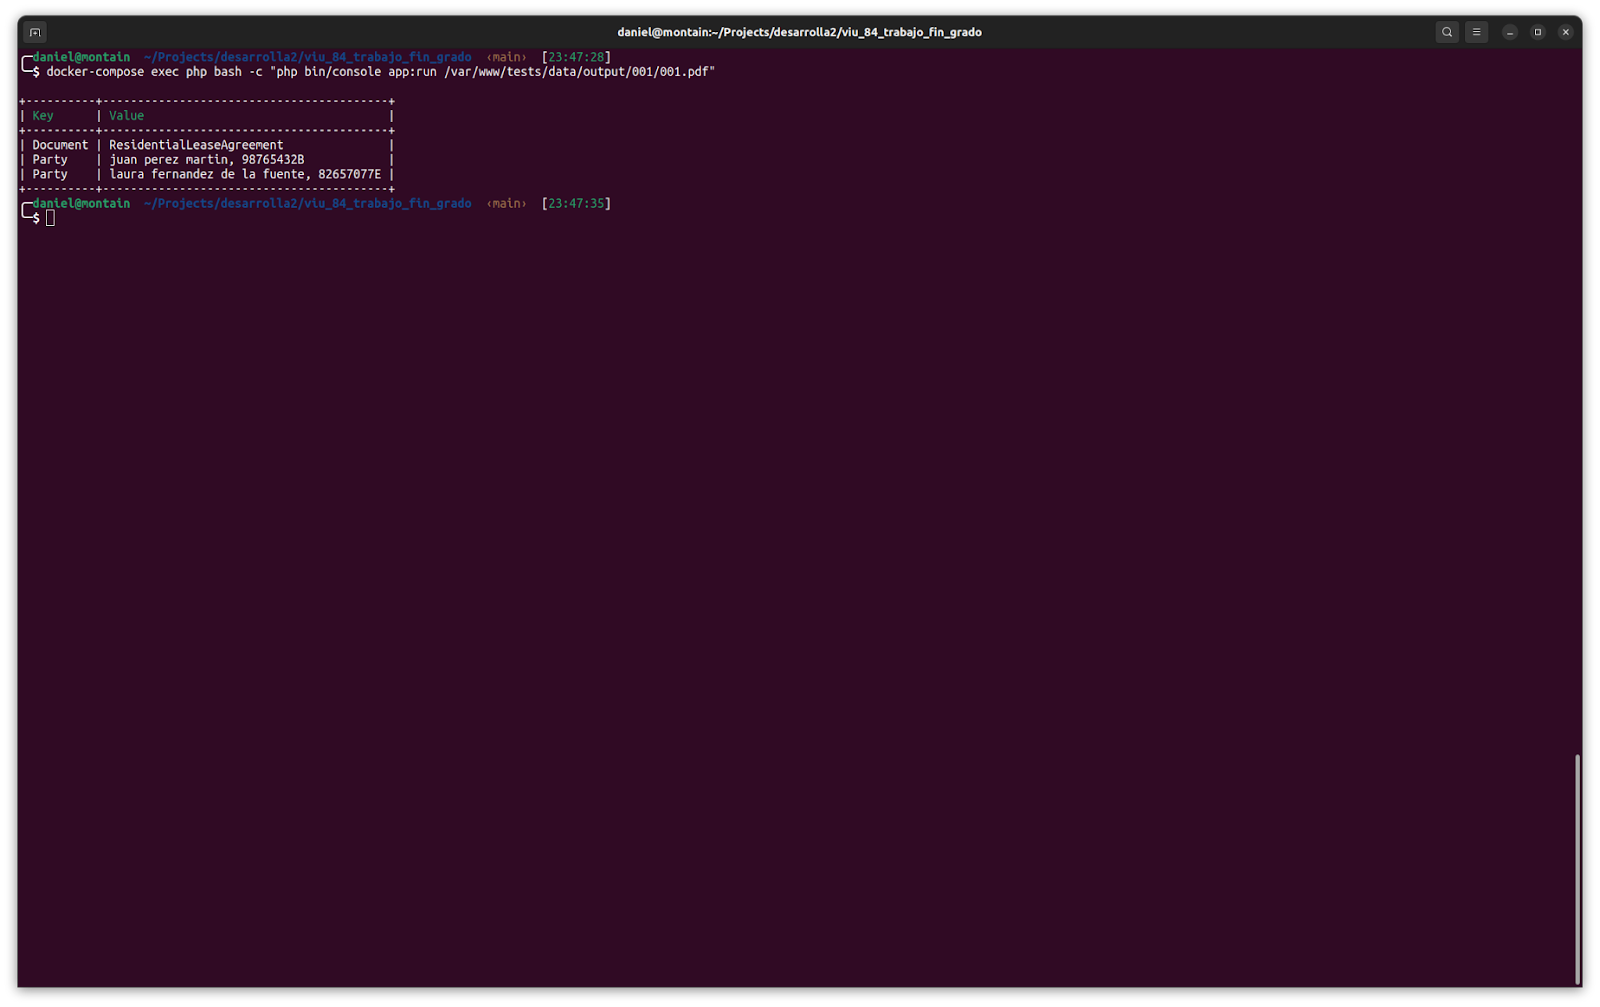
\includegraphics
    {./chapter/4/images/ad_4nxfdnwjsbh2gjzl1fmziayn8lryh5kzvpjg_3lhrv86rpzq87figcfwvjn3ilyfhdd3auhqjpie927ftvvbjujd4ezcsa-qi}
    \caption{}
    \label{fig:ad_4nxfdnwjsbh2gjzl1fmziayn8lryh5kzvpjg_3lhrv86rpzq87figcfwvjn3ilyfhdd3auhqjpie927ftvvbjujd4ezcsa-qi}
\end{figure}

Ejecución de la aplicación a través de la línea de comandos

Esta interfaz recibe como parámetro la ruta de un fichero que se pretende analizar y una vez analizado muestra una
representación en formato tabla de la información extraída del mismo.

\subsection*{Interfaz web}
La interfaz web es el principal punto de interacción para la mayoría de los usuarios. Está diseñada para ser intuitiva,
accesible y eficiente, permitiendo a los usuarios realizar una amplia gama de operaciones a través de un navegador web.

Para este proyecto hemos desarrollado una interfaz con las siguientes características

\begin{itemize}
    \item
    Diseño Responsive: La interfaz web está diseñada para ser accesible desde dispositivos de escritorio y móviles,
    asegurando una experiencia de usuario coherente y optimizada en diferentes tamaños de pantalla.
    \item
    Experiencia de usuario intuitiva: Se ha prestado atención a la usabilidad, con una interfaz limpias y fáciles de
    utilizar y retroalimentación inmediata a las acciones del usuario.
\end{itemize}

\begin{figure}
    \centering
    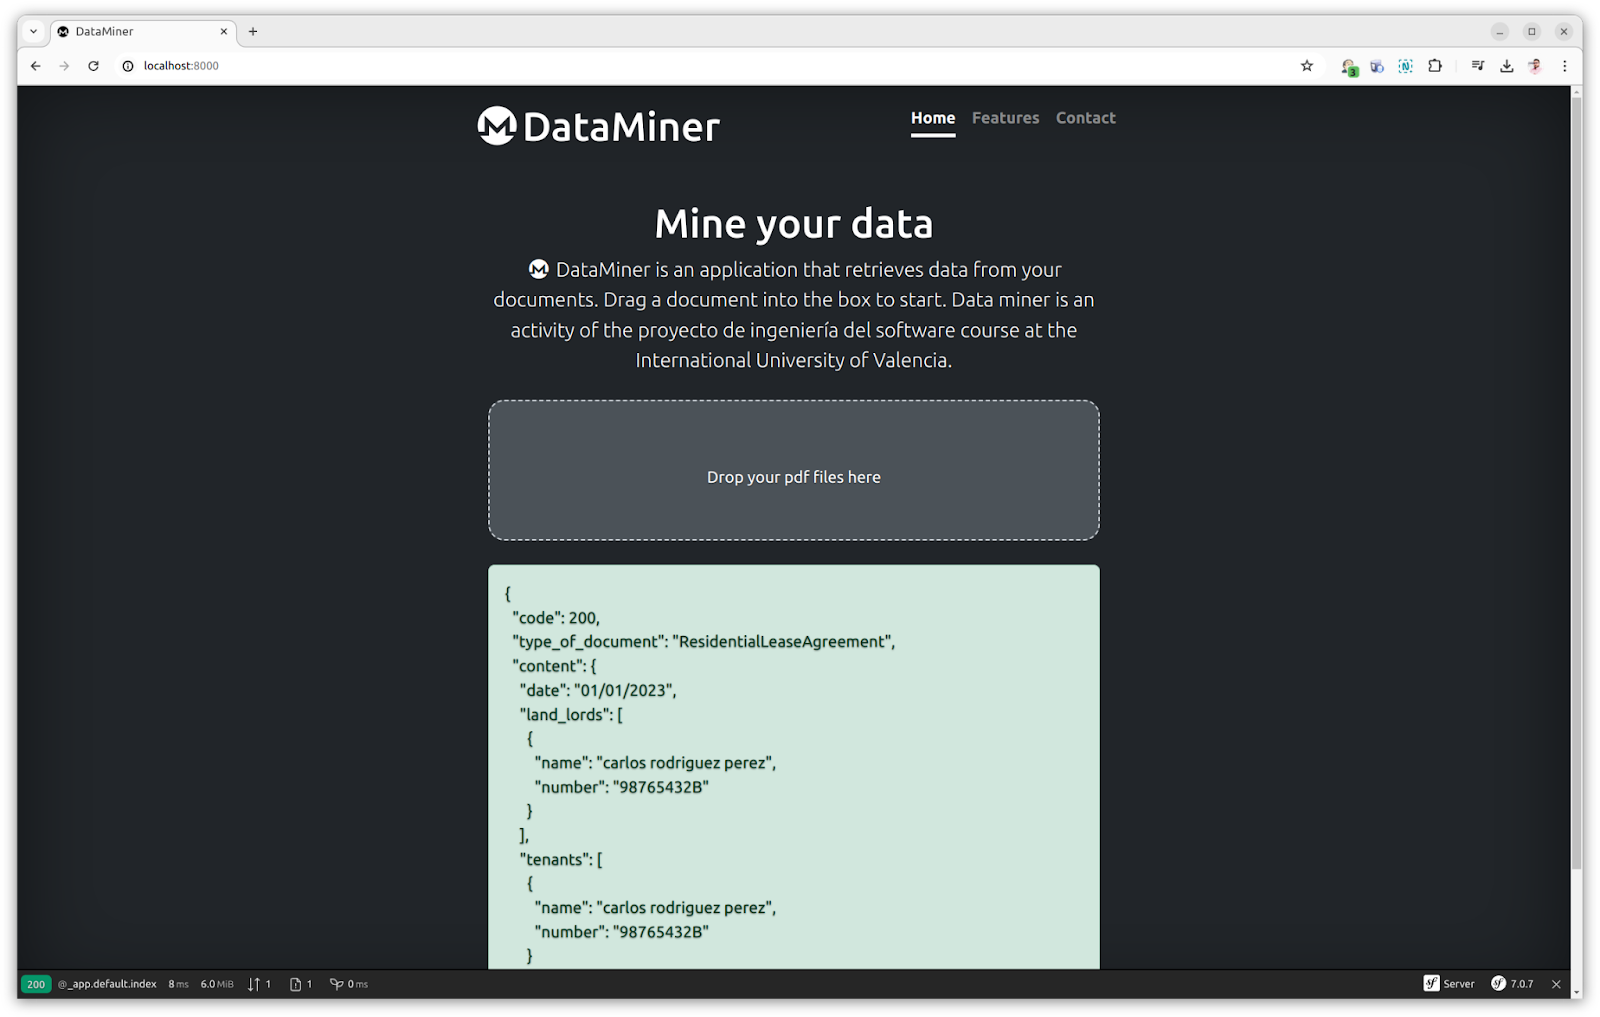
\includegraphics
    {./chapter/4/images/ad_4nxc3kwvjbdgjf8jxg_-9pf51kwcykrlcqlvr_28ejlb2jbbztkj9huiri-dti7x79w8xg3u_md1fyt0-q_gnmefljxbffub8}
    \caption{}
    \label{fig:ad_4nxc3kwvjbdgjf8jxg_-9pf51kwcykrlcqlvr_28ejlb2jbbztkj9huiri-dti7x79w8xg3u_md1fyt0-q_gnmefljxbffub8}
\end{figure}

Ejecución de la aplicación a través de la interfaz web.

Esta interfaz muestra un área sobre la que se pueden arrastrar y soltar documentos, una vez recibidos, y analizados
muestra una representación en formato json de la información extraída del mismo.

\section*{Caché}
La implementación de una caché en aplicaciones web es una técnica comúnmente utilizada para mejorar el rendimiento y la
eficiencia..

En este proyecto, la caché se ha utilizado específicamente para almacenar las peticiones HTTP realizadas, proporcionando
varias ventajas significativas, como el aumento de la velocidad de respuesta y la reducción de costos operativos..

Aunque en un entorno de producción la utilidad de esta caché podría ser limitada, en un entorno de desarrollo resulta
invaluable. Esto se debe a que en desarrollo se trabaja principalmente con un conjunto de datos más pequeño y las
peticiones se repiten con frecuencia.

\section*{Registro y gestión de logs}
El registro de logs es una parte crucial del monitoreo y mantenimiento de cualquier aplicación..

En este proyecto, se ha implementado un sistema de logging utilizando Monolog, una biblioteca de registro para PHP.

Además de los logs que almacena symfony por defecto, se han configurado 3 canales adicionales:

\begin{itemize}
    \item Generator: para los logs del componente generator.
    \item Reader: para los logs del componente reader.
    \item Http-Client: para el componente que realiza las peticiones HTTP.
\end{itemize}

Un canal es la forma en la que monolog, agrupa un conjunto de información para poderla filtrar y procesar adecuadamente.

\begin{figure}
    \centering
    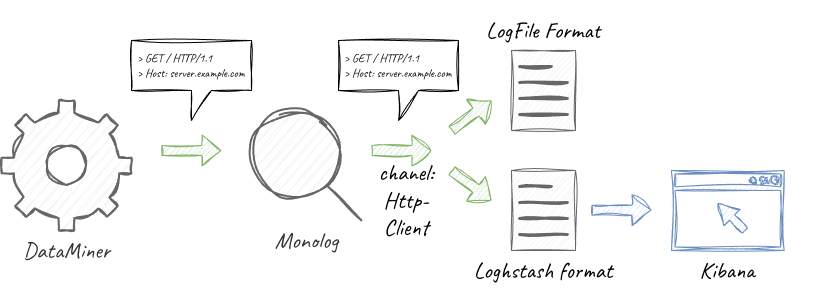
\includegraphics
    {./chapter/4/images/ad_4nxe5wisb55id7sbqcwbvoijqjbf3civblmuqf2gzkgnf2kauncps-gmu7iae0ck9ftwme-orgudhewur7els5nwraevj38i0}
    \caption{}
    \label{fig:ad_4nxe5wisb55id7sbqcwbvoijqjbf3civblmuqf2gzkgnf2kauncps-gmu7iae0ck9ftwme-orgudhewur7els5nwraevj38i0}
\end{figure}

Canal además se registra en dos ficheros diferentes

\begin{itemize}
    \item Log File format, es el formato estándar de ficheros de logs.
    \item Logstash format, es el estándar de la herramienta logstash.
\end{itemize}

\subsection*{Formato de ficheros por defecto}
El formato por defecto es adecuado para entornos de desarrollo o proyectos de pequeña envergadura. Siempre que estos
ficheros no sean demasiado grandes, se pueden trabajar a través de herramientas de línea de comandos como:

\begin{itemize}
    \item grep: Utilizado para buscar patrones específicos dentro de los archivos de logs.
    \item awk: Utilizado para procesar y analizar los logs de manera más compleja.
\end{itemize}

\subsection*{Sistema ELK}
Un sistema compuesto por Elasticsearch, Logstash y Kibana (ELK) es una solución centralizada de gestión de logs, que
permite una monitorización más avanzada de los mismos. Está indicado en entornos de producción, donde la monitorización
de logs sea una tarea importante..

\begin{figure}
    \centering
    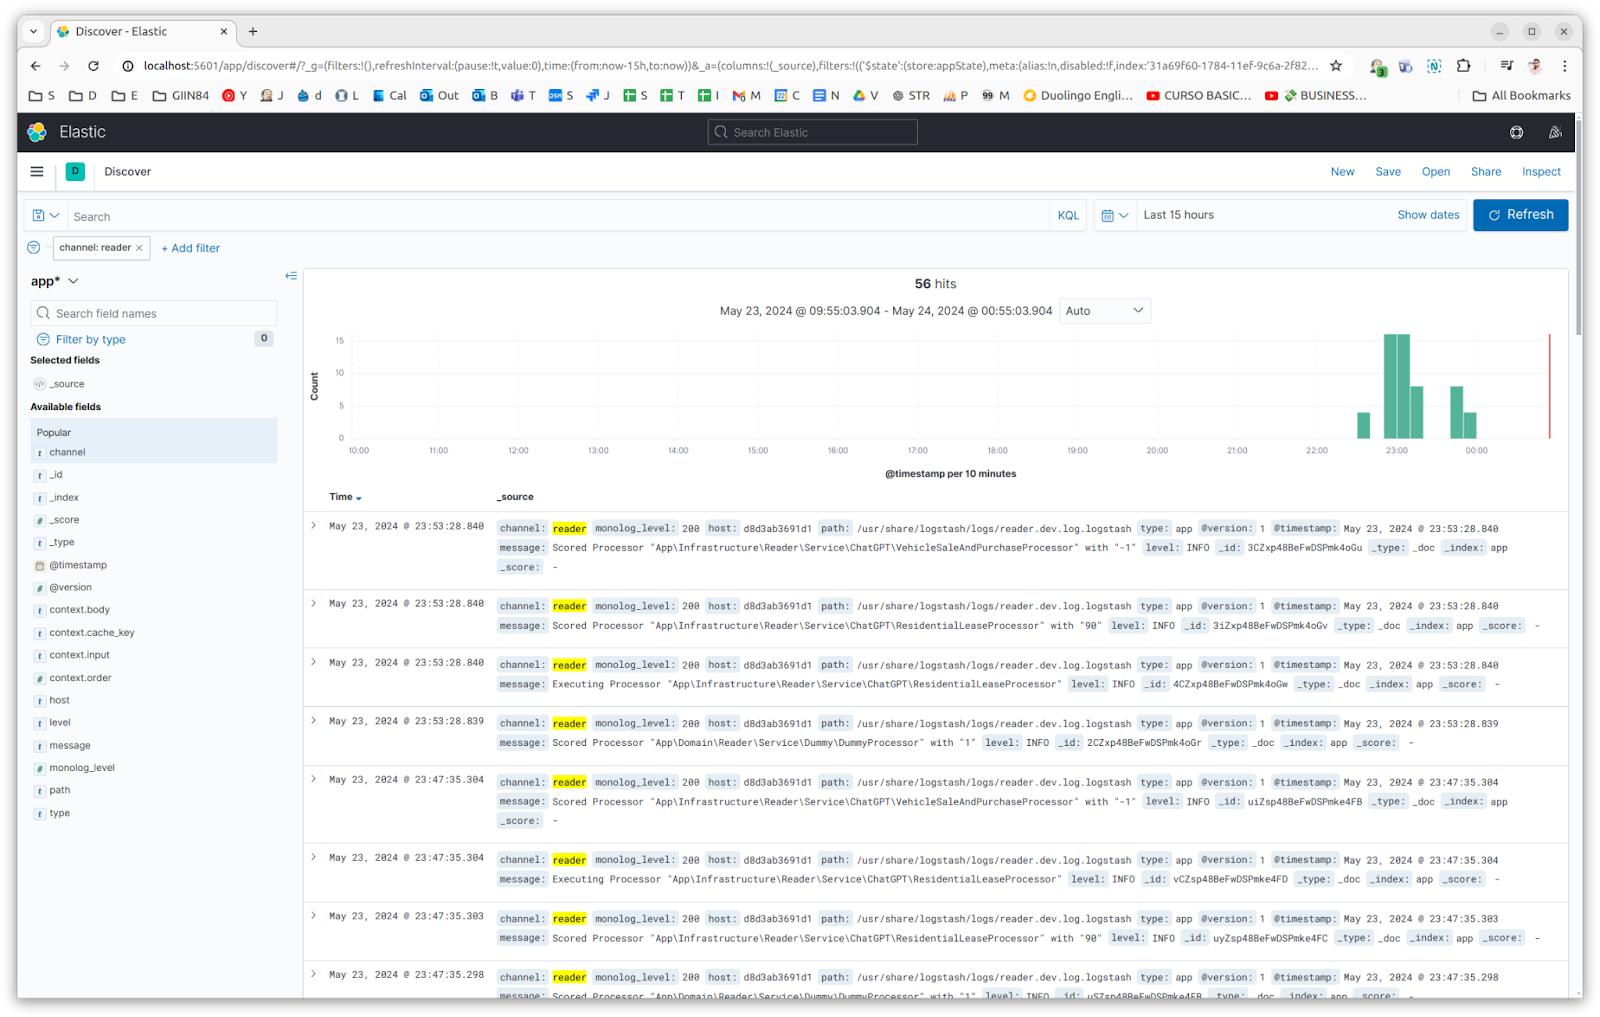
\includegraphics
    {./chapter/4/images/ad_4nxfpsnvodkc7h22x01w50v3bkprgygytiefngbdo_5-klldgxdain9x4rosk0987vpy0mkcu0gyf_art6d6y0vaw5ux1zclk}
    \caption{}
    \label{fig:ad_4nxfpsnvodkc7h22x01w50v3bkprgygytiefngbdo_5-klldgxdain9x4rosk0987vpy0mkcu0gyf_art6d6y0vaw5ux1zclk}
\end{figure}

Monitorización de logs a través de un sistema ELK

El sistema ELK se compone de tres componentes:

\begin{itemize}
    \item
    Logstash: Es una herramienta de procesamiento de datos que ingiere, transforma y envía datos a diversos destinos,
    siendo Elasticsearch uno de los más comunes.
    \item
    Elasticsearch: Es un motor de búsqueda y análisis de texto completo basado en Lucene. Permite almacenar, buscar y
    analizar grandes volúmenes de datos en tiempo real.
    \item Kibana: Es una herramienta de visualización de datos que trabaja en conjunto con Elasticsearch. Permite a los
    usuarios crear gráficos y dashboards interactivos para visualizar y analizar los datos de logs almacenados en
    Elasticsearch.
\end{itemize}

\section*{Contenedores}
La contenedorización es una técnica que permite encapsular una aplicación y sus dependencias en uno o más contenedores,
lo que garantiza que se ejecutará de manera consistente en cualquier entorno..

\subsection*{Docker}
Docker permite empaquetar la aplicación junto con todas sus dependencias en una imagen de contenedor. Esta imagen puede
ser ejecutada en cualquier máquina que tenga Docker instalado, asegurando consistencia y eliminando problemas
relacionados con diferencias en el entorno de desarrollo y producción.

En este proyecto, se ha utilizado Docker para contenerizar la aplicación, proporcionando un entorno de desarrollo y
despliegue robusto y reproducible.

\subsection*{Docker compose}
Docker Compose se utiliza para definir y ejecutar aplicaciones Docker multi-contenedor. En este proyecto, Docker Compose
gestiona la aplicación PHP junto con otros servicios necesarios, como el conjunto ELK

    \chapter{Resultados}\label{ch:chapter_5}

\begin{comment}

    El
    contenido de este apartado dependerá del tipo de trabajo de fin de
    grado llevado a cabo. Algunos aspectos que pueden incluirse son:









    \begin{itemize}

        \item
        Descripción
        detallada de la solución informática desarrollada, incluyendo sus
        características principales, funcionalidades y objetivos
        específicos.


    \end{itemize}








    \begin{itemize}

        \item
        Pruebas
        y resultados funcionales: se presentan los resultados de las pruebas
        realizadas para verificar el funcionamiento correcto de la solución.
        Muestra cómo se han llevado a cabo las pruebas y los casos de
        prueba utilizados. Destaca los resultados obtenidos en términos de
        la funcionalidad y el cumplimiento de los requisitos establecidos.


    \end{itemize}








    \begin{itemize}

        \item
        Rendimiento
        y eficiencia: evaluación del rendimiento y la eficiencia de la
        solución informática. Muestra los resultados obtenidos en términos
        de tiempos de respuesta, velocidad de procesamiento, uso de
        recursos, escalabilidad, entre otros aspectos relevantes para tu
        proyecto. Compara los resultados con los objetivos establecidos.


    \end{itemize}








    \begin{itemize}

        \item
        Evaluación
        de la usabilidad: Si la solución informática está destinada a
        usuarios finales, realiza una evaluación de la usabilidad. Utiliza
        métodos y técnicas apropiadas, como pruebas de usabilidad para
        recopilar datos sobre la experiencia del usuario. Presenta los
        resultados obtenidos y analiza la satisfacción del usuario, la
        facilidad de uso y cualquier problema identificado.


    \end{itemize}








    \begin{itemize}

        \item
        Calidad
        del código y mantenibilidad: Evalúa la calidad del código
        desarrollado y la mantenibilidad de la solución.


    \end{itemize}








    \begin{itemize}

        \item
        Casos
        de estudio o resultados específicos: Si has realizado estudios de
        casos específicos o evaluaciones particulares, describe los
        resultados obtenidos y su relevancia para tu proyecto. Puedes
        incluir ejemplos concretos de cómo la solución informática ha
        sido aplicada en situaciones reales y los resultados obtenidos en
        cada caso.


    \end{itemize}








    \begin{itemize}

        \item
        Resultados
        cuantitativos: Presenta los resultados numéricos o medibles de tu
        proyecto. Esto puede incluir métricas de rendimiento, tiempos de
        respuesta, velocidad de procesamiento, eficiencia, precisión, entre
        otros. Utiliza tablas, gráficos u otros medios visuales para
        mostrar claramente los datos recopilados.


    \end{itemize}








    \begin{itemize}

        \item
        Resultados
        cualitativos: Si tu proyecto implica evaluaciones subjetivas o
        cualitativas, como la usabilidad, la experiencia del usuario o la
        calidad percibida, describe los resultados obtenidos a través de
        encuestas, entrevistas o pruebas de usabilidad.


    \end{itemize}








    \begin{itemize}

        \item
        Validación
        y pruebas: Explica cómo se han validado y evaluado los resultados
        de tu proyecto. Si has realizado pruebas, verifica que se cumplan
        los requisitos establecidos y describe cómo se ha llevado a cabo la
        evaluación. Si se han utilizado conjuntos de datos de prueba o
        casos de uso específicos, menciónalos en esta sección.



        \item
        Comparación
        con resultados esperados: Compara tus resultados con los objetivos y
        las expectativas establecidos en la introducción de tu trabajo.
        Destaca si has logrado alcanzar tus metas y si los resultados
        obtenidos son consistentes con las hipótesis o predicciones
        iniciales. Si hay desviaciones o discrepancias, explícalas y
        proporciona posibles explicaciones.


    \end{itemize}








    \begin{itemize}

        \item
        Análisis
        de los resultados: Realiza un análisis de los resultados obtenidos
        y su relevancia para tu proyecto.


    \end{itemize}








    \begin{itemize}

        \item
        Limitaciones
        y posibles mejoras: Menciona las limitaciones o restricciones que
        puedan haber afectado tus resultados. Esto puede incluir
        limitaciones en los datos, en los métodos utilizados o en la
        implementación del proyecto. También puedes sugerir posibles
        mejoras o áreas de investigación futuras basadas en las
        limitaciones identificadas.


    \end{itemize}

\end{comment}


\section{Descripción de la solución}
El sistema desarrollado consta de una arquitectura basada en dos componentes principales: Generator y Reader.

Ambos componentes están diseñados para ser fácilmente extensibles, mediante un sistema en el que se pueden registrar
nuevos preprocesadores, procesadores y postprocesadores, para cumplir con los requisitos de casos de uso específicos.

\subsection*{Componente Generator}
El componente Generator se encarga de convertir documentos en diferentes formatos a texto plano.
En esta implementación, se desarrolló un procesador especializado que utiliza la herramienta pdftotext para transformar
documentos PDF en texto.

La arquitectura modular del Generator permite la inclusión de nuevos preprocesadores y postprocesadores para ajustar y
perfeccionar el texto generado.

\subsection*{Componente Generator}
El componente Reader interpreta y extrae la información estructurada del texto generado por el Generator.

Funciona mediante un sistema de procesadores organizados en una única capa, que opera bajo un mecanismo competitivo
similar al del componente Generator.
Los procesadores compiten entre sí para determinar cuál es el más adecuado para analizar y extraer la información
necesaria del texto.

En esta implementación, se desarrollaron dos procesadores que consumen la api pública de OpenAI, para extraer la
información de dos tipos de contratos diferentes: contratos de arrendamiento entre particulares y contratos de
compraventa de vehículos entre particulares.

\subsection*{Interfaces de Usuario}
Para interactuar con el sistema, se han desarrollado dos interfaces:

\begin{itemize}
    \item Interfaz de Línea de Comandos: Esta herramienta está dirigida a desarrolladores y
    administradores del sistema, permitiendo ejecutar comandos y scripts directamente.


    \item Interfaz Web: Presenta un área donde los usuarios pueden
    arrastrar y soltar documentos para su análisis y muestra una representación en formato JSON de la información
    extraída.
\end{itemize}


\section{Pruebas y análisis de los resultados}

\colorbox{color_highlight} {@TODO: }
explicar de nuevo que seha desarrollado una test suite de pruebas unitarias, y
completar indicando el porcentaje de acierto para las pruebas manuales.

Resultados cuantitativos: Presenta los resultados numéricos o medibles de tu
proyecto.
Esto puede incluir métricas de rendimiento, tiempos de respuesta, velocidad de procesamiento, eficiencia,
precisión, entre otros.
Utiliza tablas, gráficos u otros medios visuales para mostrar claramente los datos recopilados.

Resultados cualitativos: Si tu proyecto implica evaluaciones subjetivas o cualitativas, como la usabilidad, la
experiencia del usuario o la calidad percibida,describe los resultados obtenidos a través de encuestas, entrevistas o
pruebas de usabilidad.

Pruebas y resultados funcionales: se presentan los resultados de las pruebas realizadas para verificar el correcto
funcionamiento de la solución.

Muestra cómo se han llevado a cabo las pruebas y los casos de prueba utilizados.
Destaca los resultados obtenidos en términos de la funcionalidad y el cumplimiento de los requisitos establecidos.

Casos de estudio o resultados específicos: Si has realizado estudios de casos específicos o evaluaciones particulares,
describe los resultados obtenidos y su relevancia para tu proyecto.
Puedes incluir ejemplos concretos de cómo la solución informática ha sido aplicada en situaciones reales y los
resultados obtenidos en cada caso.

Validación y pruebas: Explica cómo se han validado y evaluado los resultados de tu proyecto.
Si has realizado pruebas, verifica que se cumplan los requisitos establecidos y describe cómo se ha llevado a cabo la
evaluación.
Si se han utilizado conjuntos de datos de prueba o casos de uso específicos, menciónalos en esta sección.

Comparación con resultados esperados: Compara tus resultados con los objetivos
y las expectativas establecidos en la introducción de tu trabajo.
Destaca si has logrado alcanzar tus metas y si los resultados obtenidos son consistentes con las hipótesis o
predicciones iniciales.
Si hay desviaciones o discrepancias, explícalas y proporciona posibles explicaciones.

Análisis de los resultados: Realiza un análisis de los resultados obtenidos y su relevancia para tu proyecto.


\section{Rendimiento}

// @TODO: Rendimiento y eficiencia: evaluación del rendimiento y la eficiencia de la solución informática.
Muestra los resultados obtenidos en términos de tiempos de respuesta,velocidad de procesamiento, uso de recursos,
escalabilidad, entre otros aspectos relevantes para tu proyecto.
Compara los resultados con los objetivos establecidos.


\section{Calidad del código}

// @TODO, Calidad del código y mantenibilidad:
Evalúa la calidad del código desarrollado y la mantenibilidad de la solución.


\section{Limitaciones}

// @TODO, Limitaciones y posibles mejoras: Menciona las limitaciones o restricciones
que puedan haber afectado sus resultados.
Esto puede incluir limitaciones en los datos, en los métodos utilizados o en la implementación del proyecto.
También puedes sugerir posibles mejoras o áreas de investigación futuras basadas en las limitaciones identificadas.


\section{Coste}
// @TODO,


\section{Posibles mejoras}

\subsection*{OCR}
\colorbox{color_highlight}{@TODO:}

\subsection*{Nuevos Readers}
// @TODO:

    \chapter{Conclusiones}\label{ch:chapter_6}


\section{Iteraciones y mejoras}
\colorbox{color_highlight}{@TODO:}

Si has realizado iteraciones o mejoras en el proceso de desarrollo, menciona los cambios realizados y las razones detrás
de ellos.

Nuestro próximo objetivo es abrir el proyecto a la comunidad, convirtiéndolo en una iniciativa de código abierto.

Esto no solo incluirá la mejora y ampliación de la documentación existente, sino también la traducción al inglés para
facilitar su adopción y contribución global.
Además, planeamos desarrollar más funcionalidades y realizar pruebas exhaustivas para asegurar la robustez y fiabilidad
del software.


\section{Teseract}

\section{Rubrica}
\colorbox{color_highlight}{@TODO:Revisar al rubrica.}




    %% Appendix
    \appendix
    \chapter{Instrucciones adicionales}\label{ch:appendix_1}


El apéndice es toda la información adicional complementaria, necesaria para ilustrar mejor el cuerpo del trabajo.

Los apéndices van numerados con una secuencia alfabética de letras mayúsculas (A, B, C, etc.). En caso de que se hayan
producido diagramas de clases, diagramas de la base de datos, casos de usos u otra información gráfica y estos no hayan
sido incluidos como parte del cuerpo del trabajo, deberán ser incluidos en la sección de apéndices.

Apéndice A

Ejemplos formatos
El estilo del párrafo tiene que ser encuadrado (justificado).
En caso de terminar con un apartado (nivel uno de título) aplicar un salto de página para comenzar siempre el siguiente
apartado en una página nueva.

Tablas

Tanto las figuras como las tablas tienen que estar indicadas en el texto y referenciadas con la numeración que tiene
asignada.
La descripción debe ser clara y explicar lo que se quiere representar con independencia de la referencia del texto.

Tanto las tablas como las figuras tendrán un estilo de párrafo centrado.
La descripción se realizará desde “Insertar título”.


Tabla 1. Operaciones matemáticas utilizadas en el estudio realizado. Elaboración propia.

Figuras

Las figuras deben estar mencionadas en el texto y ser referenciadas por su numeración Ejemplo: Se habilita un servidor
con Jupyter como se puede ver en la Figura 1, en el cual se puede disponer de diferentes kernels de programación
(Python, R, Julia…).

Figura 1.
Arquitectura Jupyter Cliente - Servidor.
Fuente: https://www.paradigmadigital.com/dev/jupyter-data-science-aplicada/


Viñetado

Está permitido el uso de viñetado:

Esta sería la forma
Segundo
En caso de tener un sub apartado
Una numeración que se quiera hacer no debe influir en la numeración de los apartados generales:

1. Item 1
2. Item 2

    \chapter{Instrucciones adicionales}\label{ch:appendix_1}


El apéndice es toda la información adicional complementaria, necesaria para ilustrar mejor el cuerpo del trabajo.

Los apéndices van numerados con una secuencia alfabética de letras mayúsculas (A, B, C, etc.). En caso de que se hayan
producido diagramas de clases, diagramas de la base de datos, casos de usos u otra información gráfica y estos no hayan
sido incluidos como parte del cuerpo del trabajo, deberán ser incluidos en la sección de apéndices.

Apéndice A

Ejemplos formatos
El estilo del párrafo tiene que ser encuadrado (justificado).
En caso de terminar con un apartado (nivel uno de título) aplicar un salto de página para comenzar siempre el siguiente
apartado en una página nueva.

Tablas

Tanto las figuras como las tablas tienen que estar indicadas en el texto y referenciadas con la numeración que tiene
asignada.
La descripción debe ser clara y explicar lo que se quiere representar con independencia de la referencia del texto.

Tanto las tablas como las figuras tendrán un estilo de párrafo centrado.
La descripción se realizará desde “Insertar título”.


Tabla 1. Operaciones matemáticas utilizadas en el estudio realizado. Elaboración propia.

Figuras

Las figuras deben estar mencionadas en el texto y ser referenciadas por su numeración Ejemplo: Se habilita un servidor
con Jupyter como se puede ver en la Figura 1, en el cual se puede disponer de diferentes kernels de programación
(Python, R, Julia…).

Figura 1.
Arquitectura Jupyter Cliente - Servidor.
Fuente: https://www.paradigmadigital.com/dev/jupyter-data-science-aplicada/


Viñetado

Está permitido el uso de viñetado:

Esta sería la forma
Segundo
En caso de tener un sub apartado
Una numeración que se quiera hacer no debe influir en la numeración de los apartados generales:

1. Item 1
2. Item 2


    \printbibliography

\end{document}
